%%%%%%%%%%%%%%%%%%%%%%%%%%%%%%%%%%%%%%%%%%%%%%%%%%%%%%%%%%%%%%%%%%%%%%%%%%%%%%%%
% simulation.tex: Chapter on ECAL Timing
%%%%%%%%%%%%%%%%%%%%%%%%%%%%%%%%%%%%%%%%%%%%%%%%%%%%%%%%%%%%%%%%%%%%%%%%%%%%%%%%
\chapter{Timing Reconstruction and Calibration}
%%%%%%%%%%%%%%%%%%%%%%%%%%%%%%%%%%%%%%%%%%%%%%%%%%%%%%%%%%%%%%%%%%%%%%%%%%%%%%%%
\section*{ECAL Timing Overview}}
An electromagnetic particle's arrival time at ECAL from proton-proton~($pp$) collisions can be measured using it's energy and time recorded by ECAL subdetector crystals.
The energy recorded by each crystal is called a \textit{hit}.  Using this hit, we can calibrate the time of each of the  75848 ECAL crystals to ensure that the arrival time of an electromagnetic particle of an event is accurately measured.
%To be able to precisely measure the arrival time, the crystals must be well calibrated. 
Crystal time calibration means defining the same reference time used by each crystal for measuring
the particle's arrival time. This can be achieved by using an electromagnetic particle like a photon, produced from a $pp$ collision
at IP, and whose trajectory or path traveled from IP to the surface of a crystal and traveling with the speed of light 
is a straight line. For such a particle, its time-of-flight~(TOF) is the ratio of the distance traveled to the speed of light.
The photon time measured by each ECAL crystal is assumed to be the same for every other crystal and defines the absolute or reference time for every other similar electromagnetic particles. The time needed to transfer the recorded signal from the front-end detectors to the back end readout electronics is also assumed to be the same for all crystals. Taking the TOF into account, we define the crystal time, $\left\langle t \right\rangle \approx 0$ as the reference time for the time measurement of the photon by each crystal.
Thus, if a crystal is properly calibrated, then the average time for hits belonging to the same event
must be zero, \ie, $\left\langle t \right\rangle_{\mbox{many hits}} \approx 0$. 
\newline
%Algorithms for extracting and calibrating ECAL crystals using the reconstructed hit~(\textit{rechit}) time have been developed
%and we describe them in detail in the coming sections.
%We use $t_{reco}$ to denote the reconstructed time of each hit or crystal.
We use for the time of an electromagnetic object like a photon, either, the time of the crystal with the highest hit energy which we
call the \textit{seed crystal} or an error weighted average or mean time of the individual time measured by crystals belonging to the photon object(a single photon is  also called a \textit{super cluster} which is made from many crystals. A supercluster can also be made of many smaller clusters called \textit{basic clusters}). The seed time is denoted $t_{seed}$ and $t_{Ave}$ is the average time.
Equation \ref{eq:AVETIME} is an expression for the average time.
%We will denote the calibrated reconstructed time of an electromagnetic object as, $T_{reco}$. 
%Measuring the difference of the ECAL measured time between any two reconstructed objects~(which can be individual crystals or electromagnetic objects) arriving from the same nominal point, which in principle are both expected to have the same time, gives a reliable measurement of the timing resolution of the sub-detector including the crystal-to-crystal synchronization factor.  In ECAL timing, the photon reconstructed time, $t_{reco}$, can be calculated using either of the following methods:
\begin{enumerate}
\item \textbf{seed time}: The time of the highest energy crystal or hit in the highest energy basic cluster~(about $9$ crystals) of the photon super cluster~(about $25$ crystals). It is denoted $t_{seed}$.
\item \textbf{Average or mean time}: This is the error weighted average time of all the crystals in the photon seed basic cluster.
It is denoted as $t_{Ave}$ or $t_{mean}$.
\begin{equation}{\label{eq:AVETIME}}
t_{Ave} = t_{mean} = \frac{\sum_{i=1}^N\frac{t_{reco, i}}{\sigma_{i}^{2}}}{\sum_{i=1}^{N}\frac{1}{\sigma_{i}^{2}}} 
\end{equation}
where $N$ is the number of crystals of the seed basic cluster of photon super cluster, $t_{reco,i}$  and $\sigma_{i}$ is the reconstructed time and uncertainty or error of the time reconstructed for each crystal respectively. 
\end{enumerate}
Therefore, the arrival time of a photon or an electromagnetic object, $t_{\gamma}$ or $t_{\Pepm}$, can either be given as $t_{seed}$ or $t_{Ave}$.
The definitions $t_{seed}$ and $t_{Ave}$ have similar performances and also advantages and disadvantages. We explore these in the analysis section of this thesis.
Before we continue, let us describe in detail how a crystal time is actually recorded by the ECAL detector. We first describe the electronics read out sequence of the ECAL and continue with how we extract the timing from the electronic signals recorded.
\section{Electromagnetic Calorimeter Readout Chain}
%%%%%%%%%%%%%%%%%%%%%%%%%%%%%%%%%%%%%%%%%%%%%%%%%%%%%%%
The ECAL electronics readout system fully described in \cite{ECALREADOUT} is a light-to-light system. Energy from an incoming electromagnetic object is absorbed and converted into scintillating light by \pb crystals. The scintillating light from these crystals is received and converted into photocurrent by Avalanche Photo-Diodes~(APD) in EB and Vacuum Photo-Triodes~(VPT) in EE. The relatively low light yield of the crystals requires a pre-amplifier which converts the photocurrent into a voltage waveform. 
This pre-amplifier also has an internal pulse shaping and the acquired pulse shape is digitized over a full dynamic range by 
a floating-point analog-to-digital~(ADC) conversion system.  
The digitized data of each signal is converted into an optical data stream which is transported off the detector through optical fibers to the upper-level off-detector where the formation of trigger tower energy sums, pipelining~(temporal storing of data until receipt of first level trigger decision) and transmission of triggered data to the data acquisition system is performed. The ECAL full readout chain can be divided into an \textit{on-detector} and \textit{off-detector} electronics. Both electronic systems are connected by 100~m radiation hard optical fiber links for transporting the optical data stream. 
%%%%%%%%%%%%%%%%%%%%%%%%%%%%%%%%%%%%%%%%%%
\newline
The on-detector electronics reads a trigger tower consisting of $5\times5$ crystals arranged in $\eta \times \phi$ grid in barrel~(EB) and $x-y$ grid in endcap~(EE).  Five Very Front End~(VFE) boards~(reading out data from 5 crystals each), one Front End board~(FE), two~(EB) and six~(EE) Giga Optical Hybrids~(GOH), one Low Voltage Regulator~(LVR) board and a Mother Board~(MB) make up the complete on-detector electronics. Electrical Signals from the APDs are accepted by the VFE equipped with a Multi-Gain Pre-Amplifier~(MGPA), a 12-bit Analogue to Digital Converter~(ADC) and a buffer. The MGPA~(an Application Specific Integrated Circuit~(ASIC) developed in 0.25~$\mu$m technology), pre-amplifies, shapes and then amplifies the signals through three amplifiers with gains of 1, 6 and 12. For the VPT~(EE), these signals first pass through a High Voltage~(HV) filter card which acts as a moderator separating very high voltages caused by the increase radiation in the EE. The full scale of the APDs and VPTs are 60~pC and 12.8~pC corresponding to $\approx$ 1.5~\TeV and 1.6-3.1~\TeV respectively. The full shaping of the signal takes about 40~ns. The noise for gain 12 is about 8000$e^{-}$ for APD configuration and about 4000$e^{-}$ for VPT configuration. 
The 3 analog output signals of the MPGA are digitized in parallel by the multichannel 40~MHz, 12-bit ADC. This ADCs have an effective number of bits of 10.9. The highest non-saturated signal is selected as the output signal and reported as 12 bits of the corresponding ADC with 2 bits coding the ADC number. It is possible, that when the signal is saturated, a wrong signal amplitude can be produced leading to some amplitude dependence of the readout time. This effect has been studied for Gains 1 and 6 transitions and the relevant correction factors for adjusting timing measurements due to this effect validated and applied.
The figures in \ref{fig:readout} is a schematics picture showing the readout chain of the FE with its MPGA and ADCs. The shaping and digitization process of a sample pulse shape~(see figure \ref{fig:pulse}) is also shown. Since the trigger decision processing requires more than one bunch crossing~(BX)(1~BX=25~ns), the signal data is pipelined during the trigger latency of 3\mus.

%%% Nice about ECAL but is it necessary here?

To protect the electronics from extreme radiating, a radiation-hard buffer adapts a low voltage differential output signal~(LVDS) of the ADC to input into the FE. Signals from  five  identical channels are integrated and read into VFE card with a Detector Control Unit for measuring APD leakage currents. The noise from each VFE is typically 1.1, 0.75, 0.6 ADC counts for gains 12, 6 and 1 respectively. This would be about 40~MeV for gain 12.
Digitized data from 5 VFE cards are fed into each FE through the LVDS and stored in 256-word-deep dual-ported memories called pipelines. Data pipelines can be stored for up to 128 bunch crossings. The FE is base on a ASIC called FERNIX holding and the logic is to calculate the energy of 5 channels once every bunch crossing. This energy is summed in strips of 5 crystals  along $\phi$. This means each VFE is serviced by a FERNIX chip. In the case of the EE, the five strip energy sum are transported by GOH to the off-detector electronics Trigger Concentration Card~(TCC) while for EB, there is a sixth FERNIX which sums the five strips energy sums and calculates an electromagnetic bit which is used to identify electromagnetic shower candidates on the basis of their shower profile in a trigger tower. The trigger tower~($5\times5$ crystals) energy sums and the electromagnetic bit is transmitted to the TCC through the GOH. This process is referred to as Trigger Primitive Generation~(TPG). Once a Level-1 trigger signal is received, the ten 40~MHz samples for each channel are transmitted to the off-detector electronics Data Concentration Card~(DCC) using an identical GOH. This takes about 7.5~$\mu$s. The VFE and FE cards are controlled using a 40~MHz digital optical link system controlled by the off-detector Clock and Control System~(CCS). 
\newline
The Off-detector electronics consist of different types of electronic boards~(the Clock and Control System~(CCS), Trigger Concentration Card~(TCC) and Data Concentration Card~(DCC) modules) sitting in an 18 VME-9U crates and a 1 VME-6U crate holding the Selective Read-Out Processor~(SRP). This system is serving both the trigger and the  Data Acquisition Systems~(DAQ) paths. In the DAQ path, the DCC performs data read-out and data reduction based on flags of the SRP. While in the trigger path, at each bunch crossing, the trigger primitive generation which began in the FE is finalized and synchronized or time aligned in the TCC before being transmitted to the regional calorimeter triggers. The trigger primitives each referring to a single trigger tower~(25 crystal data) consists of the summed transverse energy deposits and the electromagnetic bit characterizing the lateral shower profile of the electromagnetic shower. The accepted signal for accepted events is returned from the global trigger after about 3~$\mu$s and the selected events are read into the data acquisition system to the filter farm where the even rate is further reduced using data from the full detector.

In the regional calorimeter, the ECAL trigger primitives together with the HCAL trigger primitives are used to  compute the electron/photon and jet candidates as well as their transverse energy. The resulting physics objects after passing through the HLT trigger are transferred to the various tier systems for offline full event reconstruction. The ECAL also has a laser calibration systems where laser light is delivered directly to the \pb crystals using optical fibers. The laser data is used for energy and time calibration of crystals and hardware system. The crystals are energy calibrated because of the decrease in optical transmission due to the formation of color centers in the crystal. The formation of color centers is caused by irradiation. Time calibration using laser data can be performed in case there are hardware timing offset especially during long short down maintenance period of the CMS detectors.
%%%% ECAL Readout Electronics
\begin{center}
\centering
\mbox{
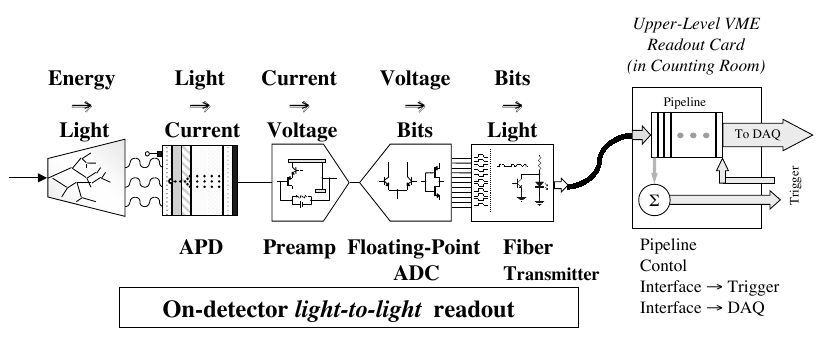
\includegraphics[height=0.5\textwidth, width=0.50\textwidth]{THESISPLOTS/CMS-ECAL-READOUT-CHAIN.png} \quad
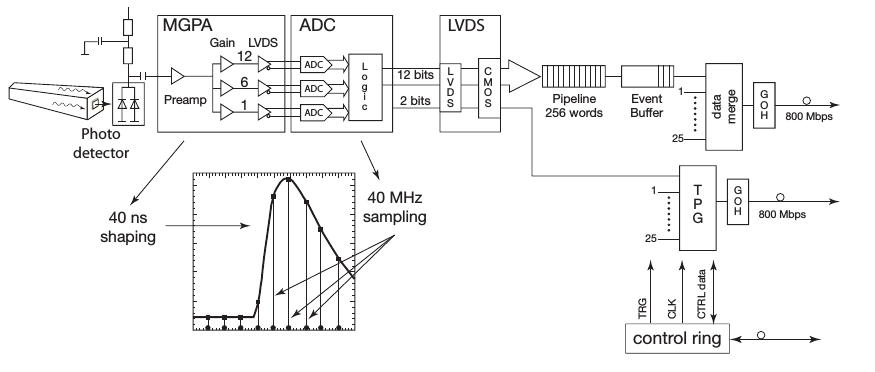
\includegraphics[height=0.5\textwidth, width=0.450\textwidth]{THESISPLOTS/ReadOut.png}
} 
\captionof{figure}{Schematic diagram of the CMS ECAL ReadOut Chain.}
\label{fig:readout}
\end{center}


\begin{center}
\centering
\mbox{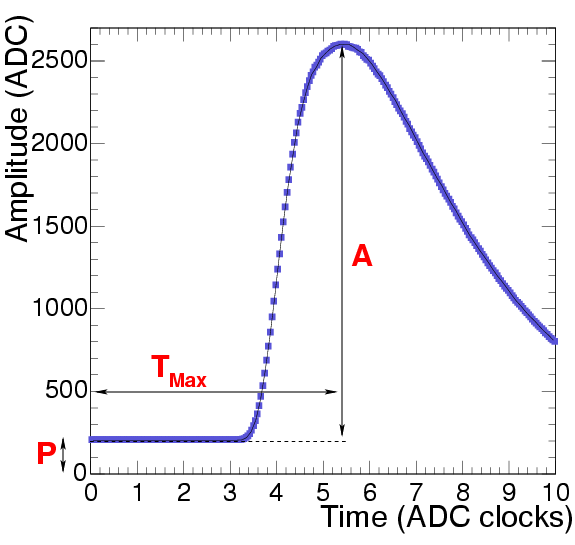
\includegraphics[height=0.5\textwidth, width=0.5\textwidth]{THESISPLOTS/Time_Amplitude_Profile.png}}
%\mbox{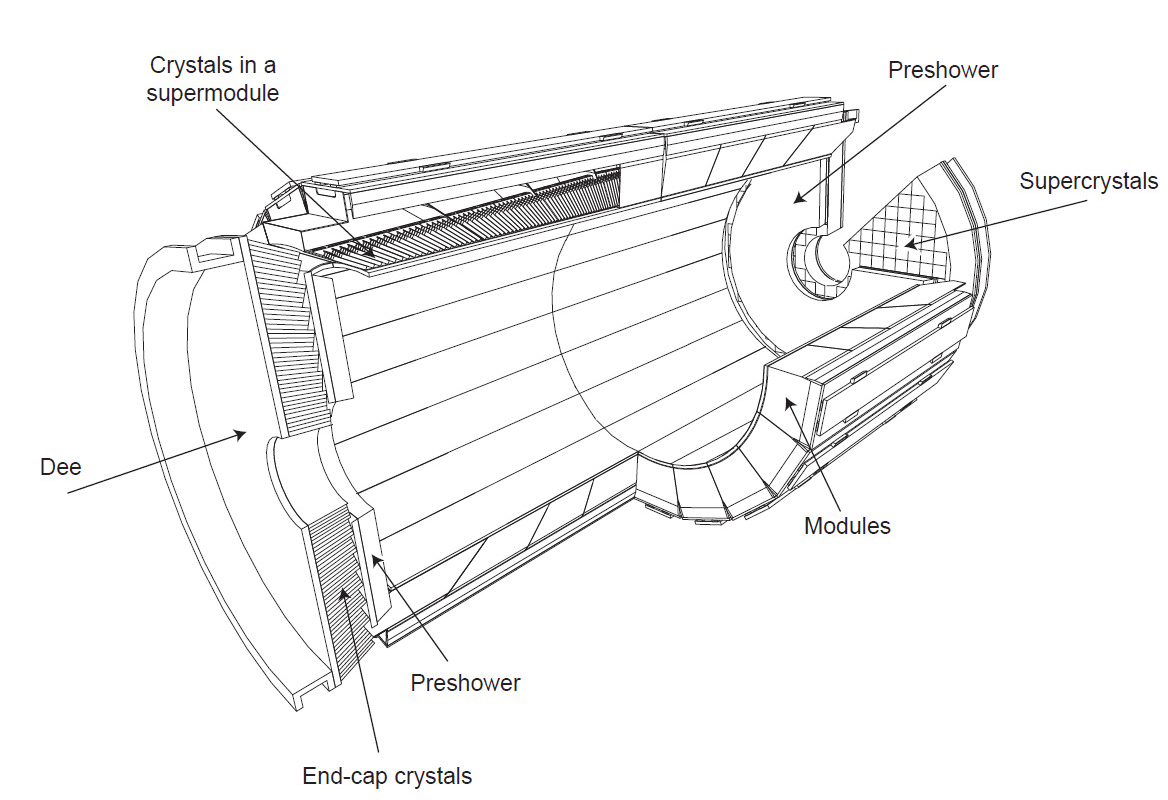
\includegraphics[scale=0.2]{THESISPLOTS/CMS-ECAL.png}}
%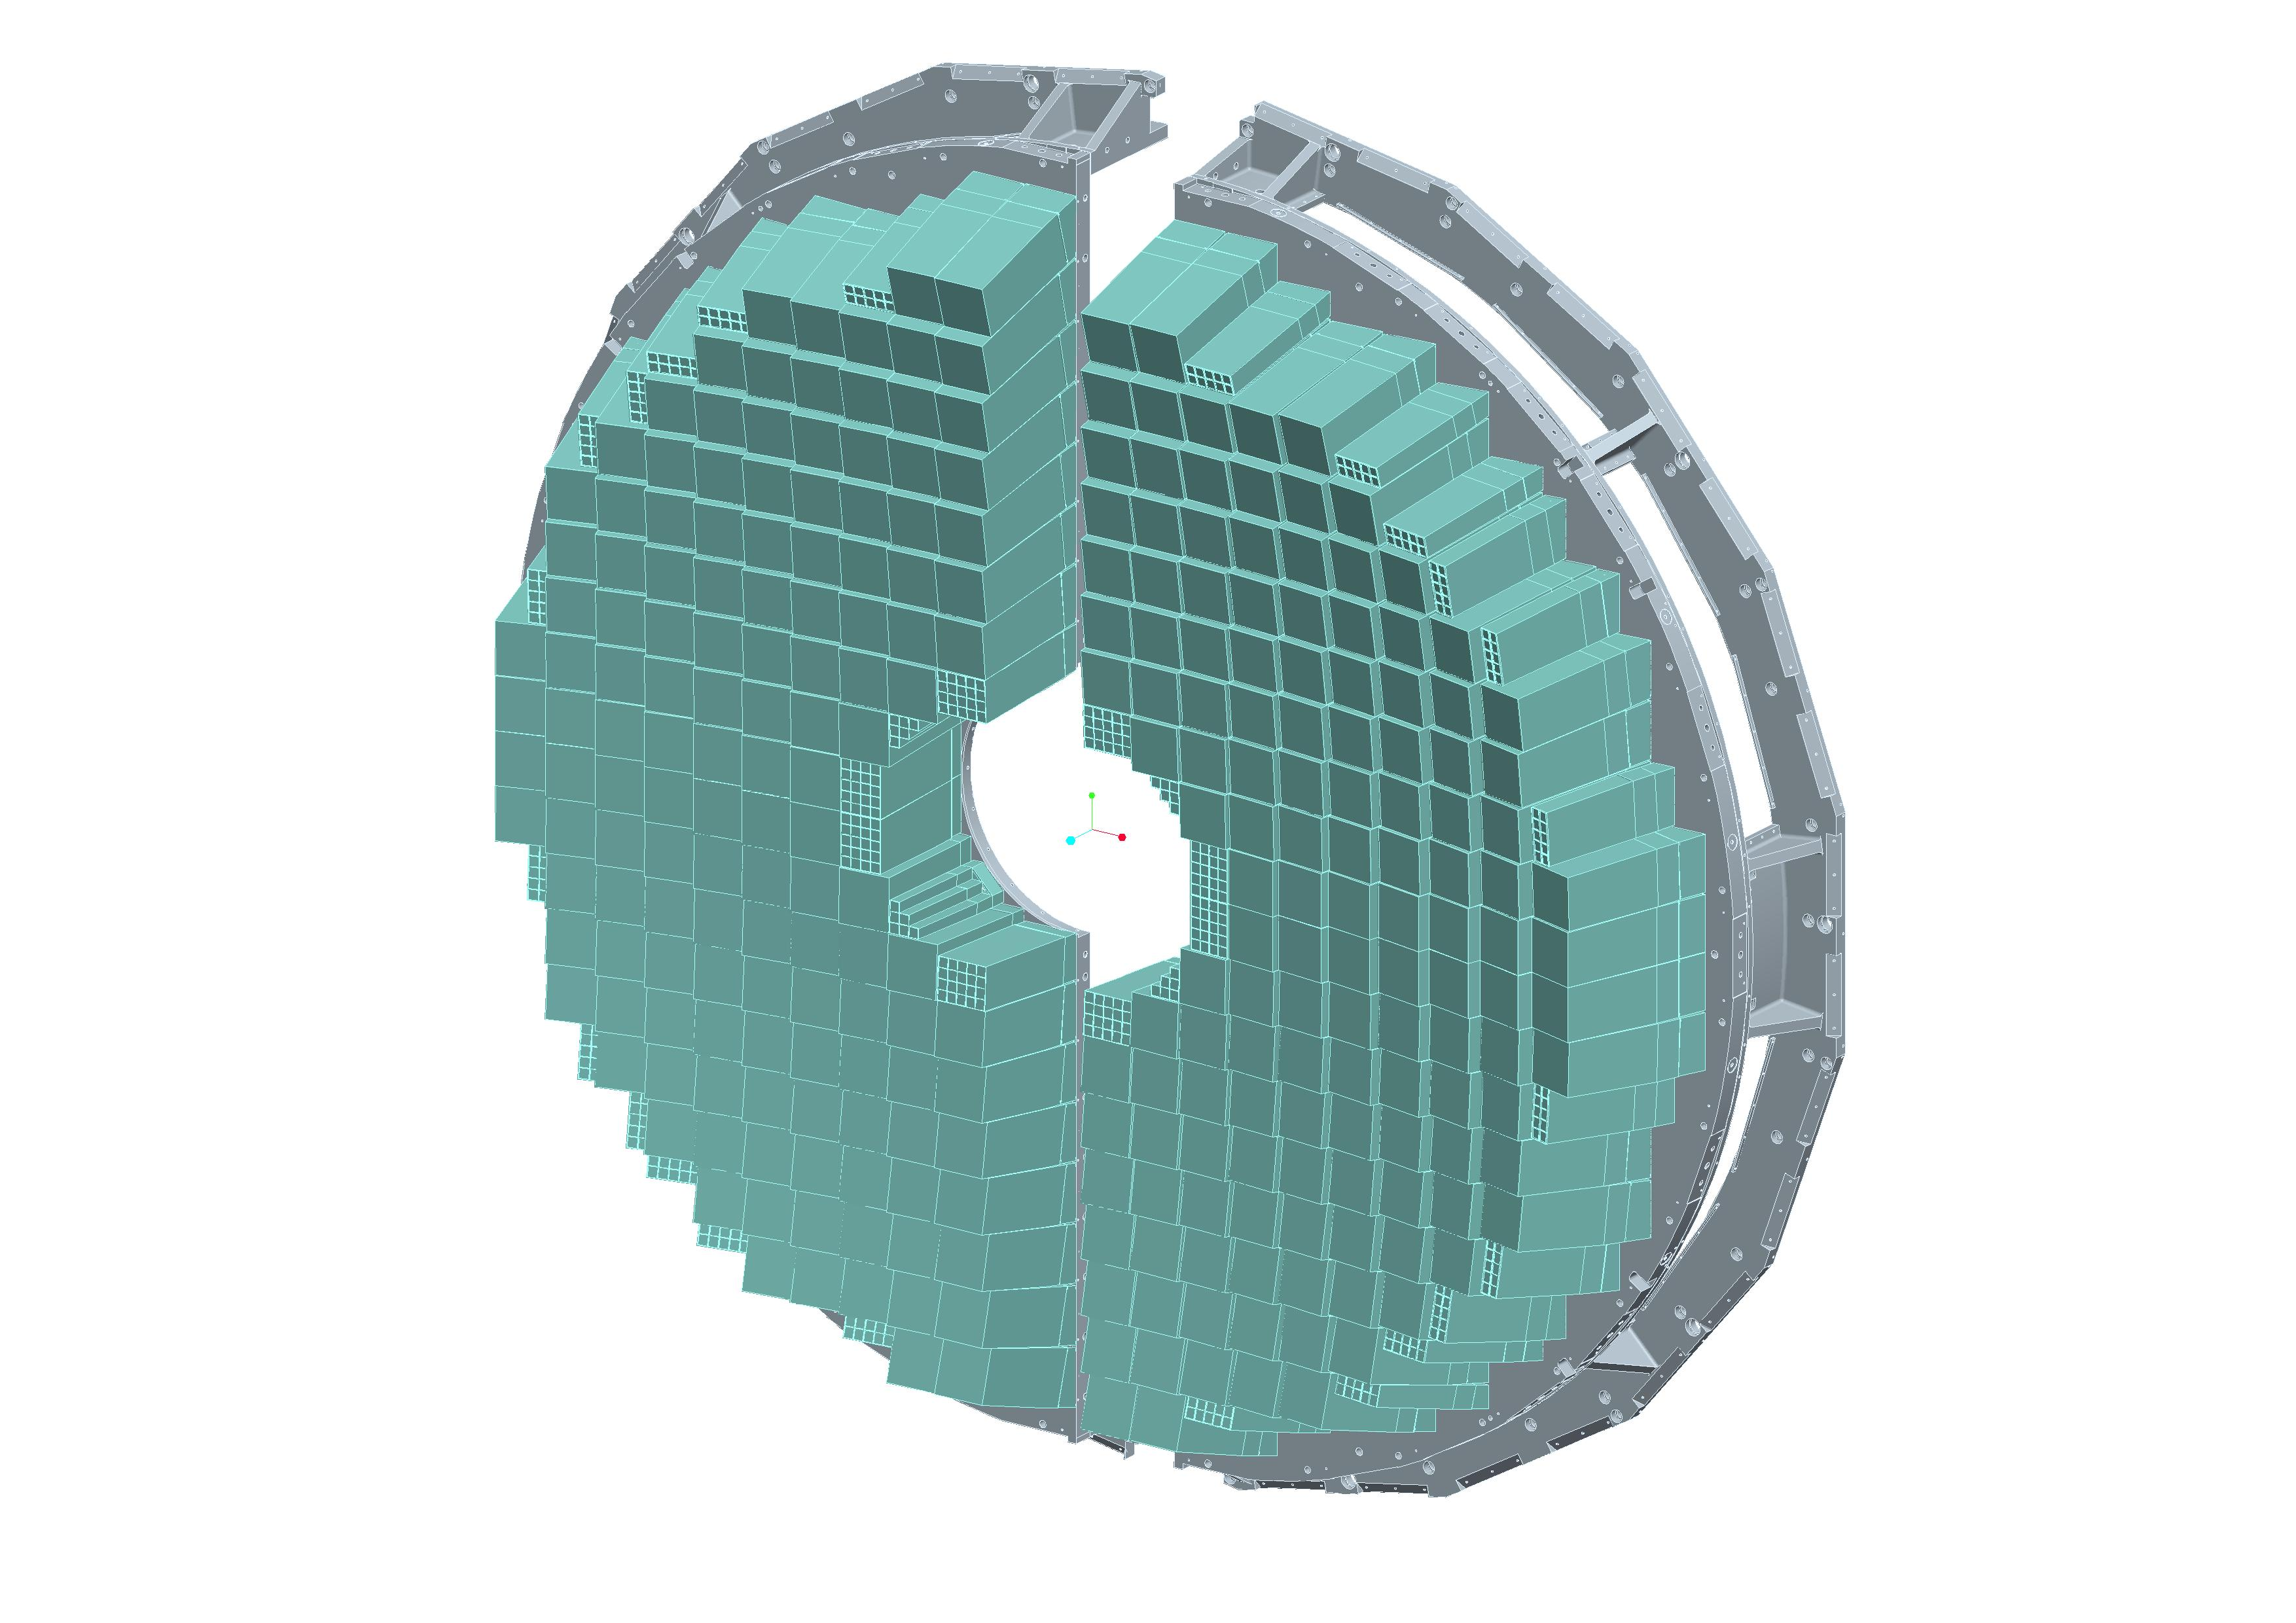
\includegraphics[scale=0.06]{THESISPLOTS/endcap_CMS.png}} 
\captionof{figure}{Typical pulse shape of a given signal showing crystal signal.}
\label{fig:pulse}
\end{center}

 %%%%%%%%%%%%%%%%%%%%%%%%%%%%%%%%%%%%%%%%%%%%%%%%%%%%%%%%%%%%%%%%%%%%%%%%%%%%%%%%
\section{Timing Extraction}
%%%%%%%%%%%%%%%%%%%%%%%%%%%%%%%%%%%%%%%%%%%%%%%%%%%%%%%%%%%%%%%%
%Anlog signals from the APD/VPT of a single crystal is preamplified producing a typical signal pulse shown in figure \ref{fig:pulse}. 

Using the pulse shape from a single crystal produced by an arriving photon or electron, the photon's energy deposited on each crystal is obtained from the amplitude of the pulse shape while it's arrival time is extracted using 10 samples created by sampling the pulse shape with an ADC clock of sampling frequency, 40~MHz. The distribution of these 10 samples along the pulse shape is shown in the left plot in figure \ref{fig:amplVsTmax}.  
The value \textbf{P} in figure \ref{fig:pulse} is the pedestal or noise read in ADC counts in the absence of a signal. 
A timing algorithm is employed to extract the time. The objective of this algorithm is to use the maximum amplitude value of the pulse, $\mathbf{A_{MAX}}$, and its corresponding time value of the ADC time, $\mathbf{T_{MAX}}$ to reconstruct an event time. 
%Thus, ECAL timing reconstruction is using the 10 samples of the pulse amplitude to measure $\mathbf{T_{MAX}}$.
Finding the true $\mathbf{A_{MAX}}$ is archived using an energy reconstruction algorithm.
Extracting of the arrival time is by comparing the pulse shape of a channel obtained during proton-proton collision to a reference pulse shape obtained during early LHC \textit{test beam} results.
This reference pulse shape has been obtained from  measurements using synchronous LHC events. Figure \ref{fig:amplVsTmax}(\textit{Left}) shows a distribution of $A/\mathbf{A_{MAX}}$ on the vertical axis against $T - \mathbf{T_{MAX}}$ on the horizontal axis obtained from test beam experiments. $T$ is an arbitrary time  measurement and $\mathbf{T_{MAX}}$ is the time when the  pulse reaches its maximum value, $\mathbf{A_{MAX}}$.


\begin{center}
\centering
\mbox{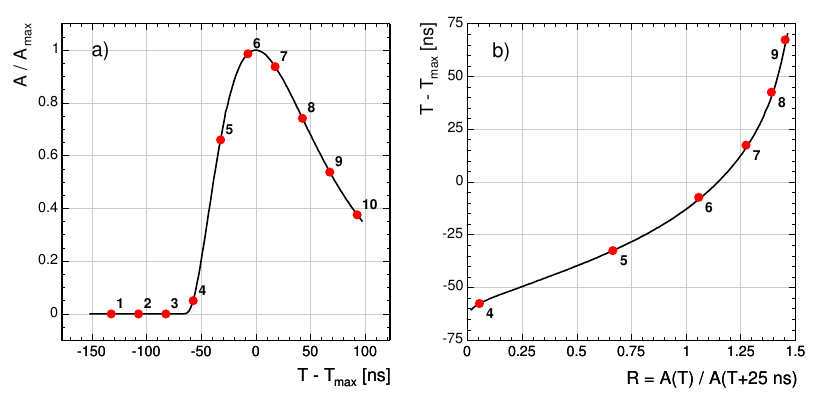
\includegraphics[height=0.45\textwidth, width=0.45\textwidth]{THESISPLOTS/AmplitudeVsTMax.png}
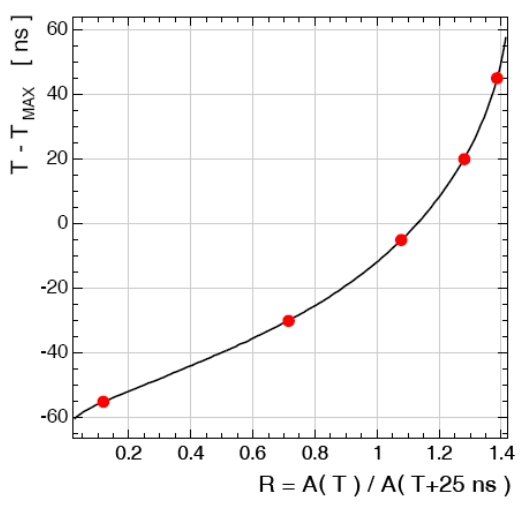
\includegraphics[height=0.45\textwidth, width=0.45\textwidth]{THESISPLOTS/TMaxPhaseVsRatio.png}}
%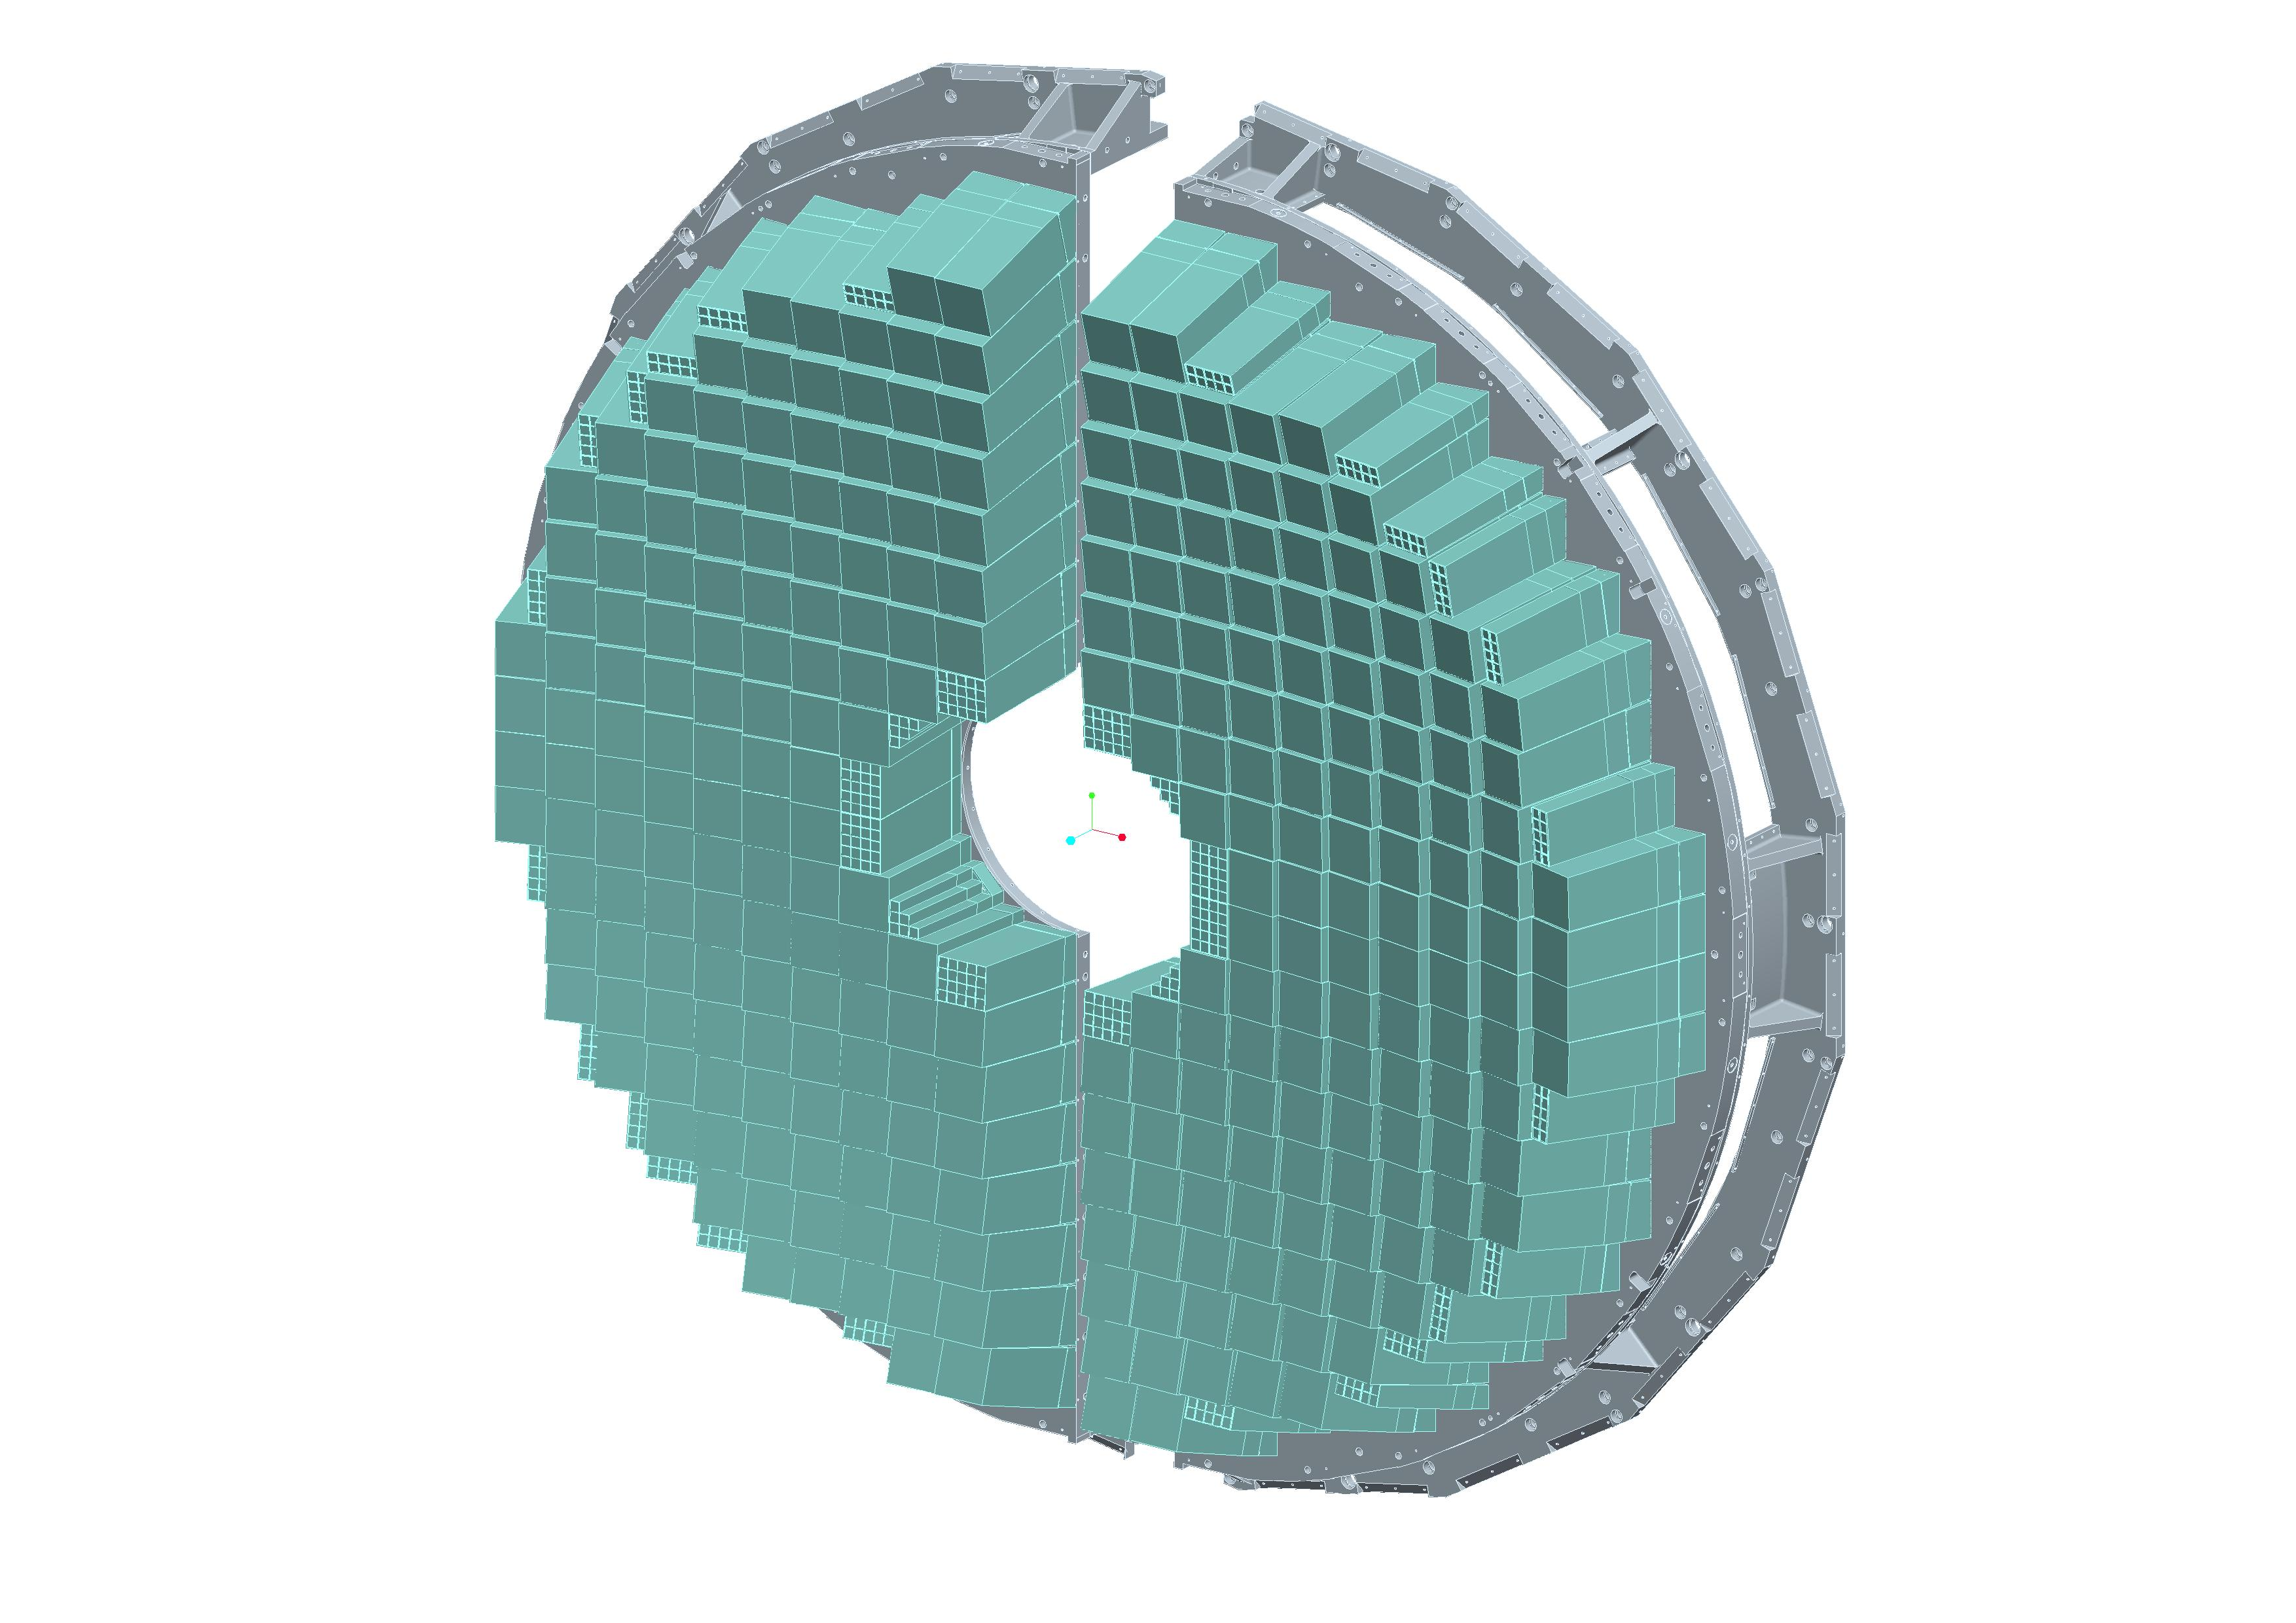
\includegraphics[scale=0.06]{THESISPLOTS/endcap_CMS.png}} 
\captionof{figure}{\textit{Left}: A measured ECAL pulse shape for a single channel. \textit{Right}: $T - T_{MAX}$ Vs $ R(T)$ showing the distribution of $T(R)$. Solid line is reference shape or shape from test beam while dots correspond to a 10 discrete samples corresponding to signal from proton-proton collision. }
\label{fig:amplVsTmax}
\end{center}
The test beam comparison is realized through an analytic fit to the 10 digitized samples. However, performing this fit directly on the $A(T)$ distribution to obtain $\mathbf{A_{MAX}}$ and $\mathbf{T_{MAX}}$ is cumbersome and technically inefficient since the amplitude of each sample depends on the pulse shape, the $\mathbf{A_{MAX}}$ value and also the relative position of $\mathbf{T_{MAX}}$ between each sample point. This relative position or phase is referred to as "\textit{$T_{MAX}$ phase}". In order to minimize the fit dependence on $A_{MAX}$ and the $T_{MAX}$ phase, a new variable not sensitive to this phase, defined as, $R(T) = A(T)/ A(T + 25~\mbox{ns})$, is used and the analytic fit is performed on the distribution of $T - T_{MAX}$ against $ R(T)$. This  $T(R)$ distribution is independent of $A_{MAX}$ and can be very well described using a polynomial of order $7$. A distribution of $T(R)$ is shown in figure \ref{fig:amplVsTmax}(\textit{Right}) with both the four to five samples points~(dots) obtained from the ratio $R_{i} = A_{i}/A_{i+1}$ from each consecutive pair of samples and the reference pulse shape~(continuous line). Each point $R_{i}$ gives a quick accurate measurement of $T_{MAX,i} = T_{i} - T(R_{i})$. The uncertainty, $\sigma_{i}$, on each measurement is a product of the derivative of the function $T(R)$ and the uncertainty on the value of $R_{i}$. The uncertainty on the value of $R_{i}$ depends on three separate uncertainties: the noise fluctuation, $\sigma_{n}$ of each sample, the uncertainty in the estimation of the pedestal value which is always subtracted from the measured value and the truncation during 12-bit digitization. These uncertainties are uncorrelated and can be added in quadrature.
The reconstructed time and its error of a hit~(fraction of energy deposited on a single crystal) is determine according to equation \ref{eq:TMAX} by taking into consideration the different uncertainties, $\sigma_{i}$ of each point,$R_{i}$.


\begin{equation}{\label{eq:TMAX}}
\displaystyle{T_{MAX} = \frac{\sum \frac{T_{MAX,i}}{\sigma^{2}_{i}}}{\sum \frac{1}{\sigma^{2}_{i}}}} \quad ; \quad\quad
\displaystyle{\frac{1}{\sigma^{2}_{T}} =  \sum \frac{1}{\sigma^{2}_{i}} }
\end{equation}
The sum is over all the 4 or 5 $R_{i}$ ratios and the assumption is that the weights are uncorrelated. 

%%%%%%%%%%%%%%%%%%%%%%%%%%%%%%%%%%%%%%%%%%%%%%%%%%%%%%%%%%%
\section{Timing Resolution}
%%%%%%%%%%%%%%%%%%%%%%%%%%%%%%%%%%%%%%%%%%%%%%%%%%%%%%%%%%%
Using the reconstructed time for each channel, $\mathbf{T_{MAX}}$, we  can measure how reliable is using the ECAL detector
to measure the arrival time of a photon or electron. This reliability can be quantified using the \textit{timing resolution}, $\sigma(t)$. The timing resolution for ECAL can be parametrized and expressed as a sum in quadrature~(uncorrelated) of three major terms contributing to the uncertainty in time measurement. These three contributions are: First, the \textit{Noise}~($N$) term, from electronic noise, coherent movement of the baseline and effects arising in addition to the main or hard proton-proton collision, other soft or less energetic collision producing events called \textit{pile up}~(PU) events. Second, the \textit{Stochastic} term~($S$), from fluctuations in the photon collection time because of the finite time during \pb scintillation. Finally the \textit{Constant} term~($C$) whose contribution is independent of the energy deposited but rather from effects correlated with the point of shower initiation within the crystal and systematics in the extraction of the time due to different pulse shape for each channel.
The timing resolution, $\sigma(t)$, with all these parameters can be expressed as given in equation \ref{eq:TimeRes}.

\begin{equation}{\label{eq:TimeRes}}
\sigma^{2}(t) = \left(\frac{N}{A/ \sigma_{n}}\right)^{2} + \left(\frac{S}{\sqrt{A}}\right)^{2} + C^{2}
\end{equation}
$A$ is the measured amplitude corresponding to the energy deposited and $\sigma_{n}$ is the intrinsic noise for individual channel. $\sigma_{n}$ has a value of $\approx 42$~MeV and $140$~MeV in the barrel and endcap respectively. $N = 33$~ns has been measured from Monte Carlo~(MC) simulation studies. Contribution from the stochastic term, ($S$) is considered small, with value of $S < 7.9$~ns$\cdot MeV^{1/2}$.
\newline
To measure the timing resolution, a simple experiment was performed in which electron beams with energies between $15$~GeV(GeV = Giga electron volts = $10^{6}$~eV, 1~eV$ = 1.602 \times 10^{-19}$~joules~(J) in energy units) and $250$~GeV was directed unto each crystal in a supermodule. The timing resolution measurement is obtained by extracting from the measured distribution of the difference in timing between two crystals sharing energy and from the same electromagnetic shower. The advantage of this approach is that, the contribution from poor synchronization is less as synchronization effects do not affect the spread. The average time method was not used as it is affected by synchronization effects. %However, there are still crystal-to-crystal synchronization effects.
There are other studies where the time difference between two groups of crystals, about, $5\times5$  crystals called basic clusters of an  electromagnetic shower was used.

Neglecting the stochastic term since its contribution is negligible, the timing resolution from two objects~(crystals or basicclusters) can be expressed as given in equation \ref{eq:TIMERES}. It is this approach which we employ in future studies of the ECAL timing resolution.
 
 \begin{equation}{\label{eq:TIMERES}}
 \sigma^{2}(t_{1} - t_{2}) = \left(\frac{N}{A_{eff}/ \sigma_{n}}\right)^{2} + 2\bar{C}^{2}
 \end{equation}
 
In equation \ref{eq:TIMERES}, $A_{eff} = A_{1}A_{2}/\sqrt{A^{2}_{1} + A^{2}_{2}}$, $t_{1,2}$ and $A_{1,2}$ correspond to the times and amplitudes of the two objects and $\bar{C}$ is their residual contribution.
We measure the timing resolution by using the standard deviation of a Gaussian fit to the time distribution from each slice in $A_{eff}/\sigma_{n}$ distribution. The resulting distribution of $\sigma(t_{1} - t_{2})$  of the extracted standard deviation of each slice against $A_{eff}/\sigma_{n}$ is fitted to extract the noise and constant term.  The result is shown in Figure \ref{fig:FitTimeRes}. The noise factor $N = (35.1 \pm 0.2)$~ns and $\bar{C} = (20 \pm 4)$ ~ns from the fit gives the values measured from the test beam experiment. 

\begin{center}
\centering
\mbox{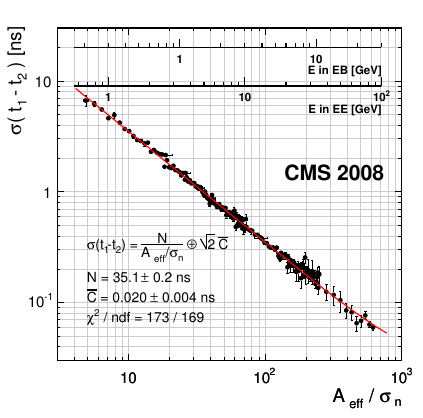
\includegraphics[height=0.6\textwidth, width=0.7\textwidth]{THESISPLOTS/ECAL_Timing_Resolution.png}}
%\mbox{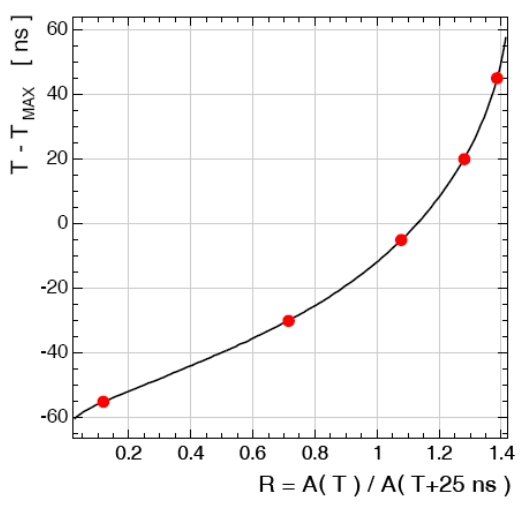
\includegraphics[scale=0.45]{THESISPLOTS/TMaxPhaseVsRatio.png}}
%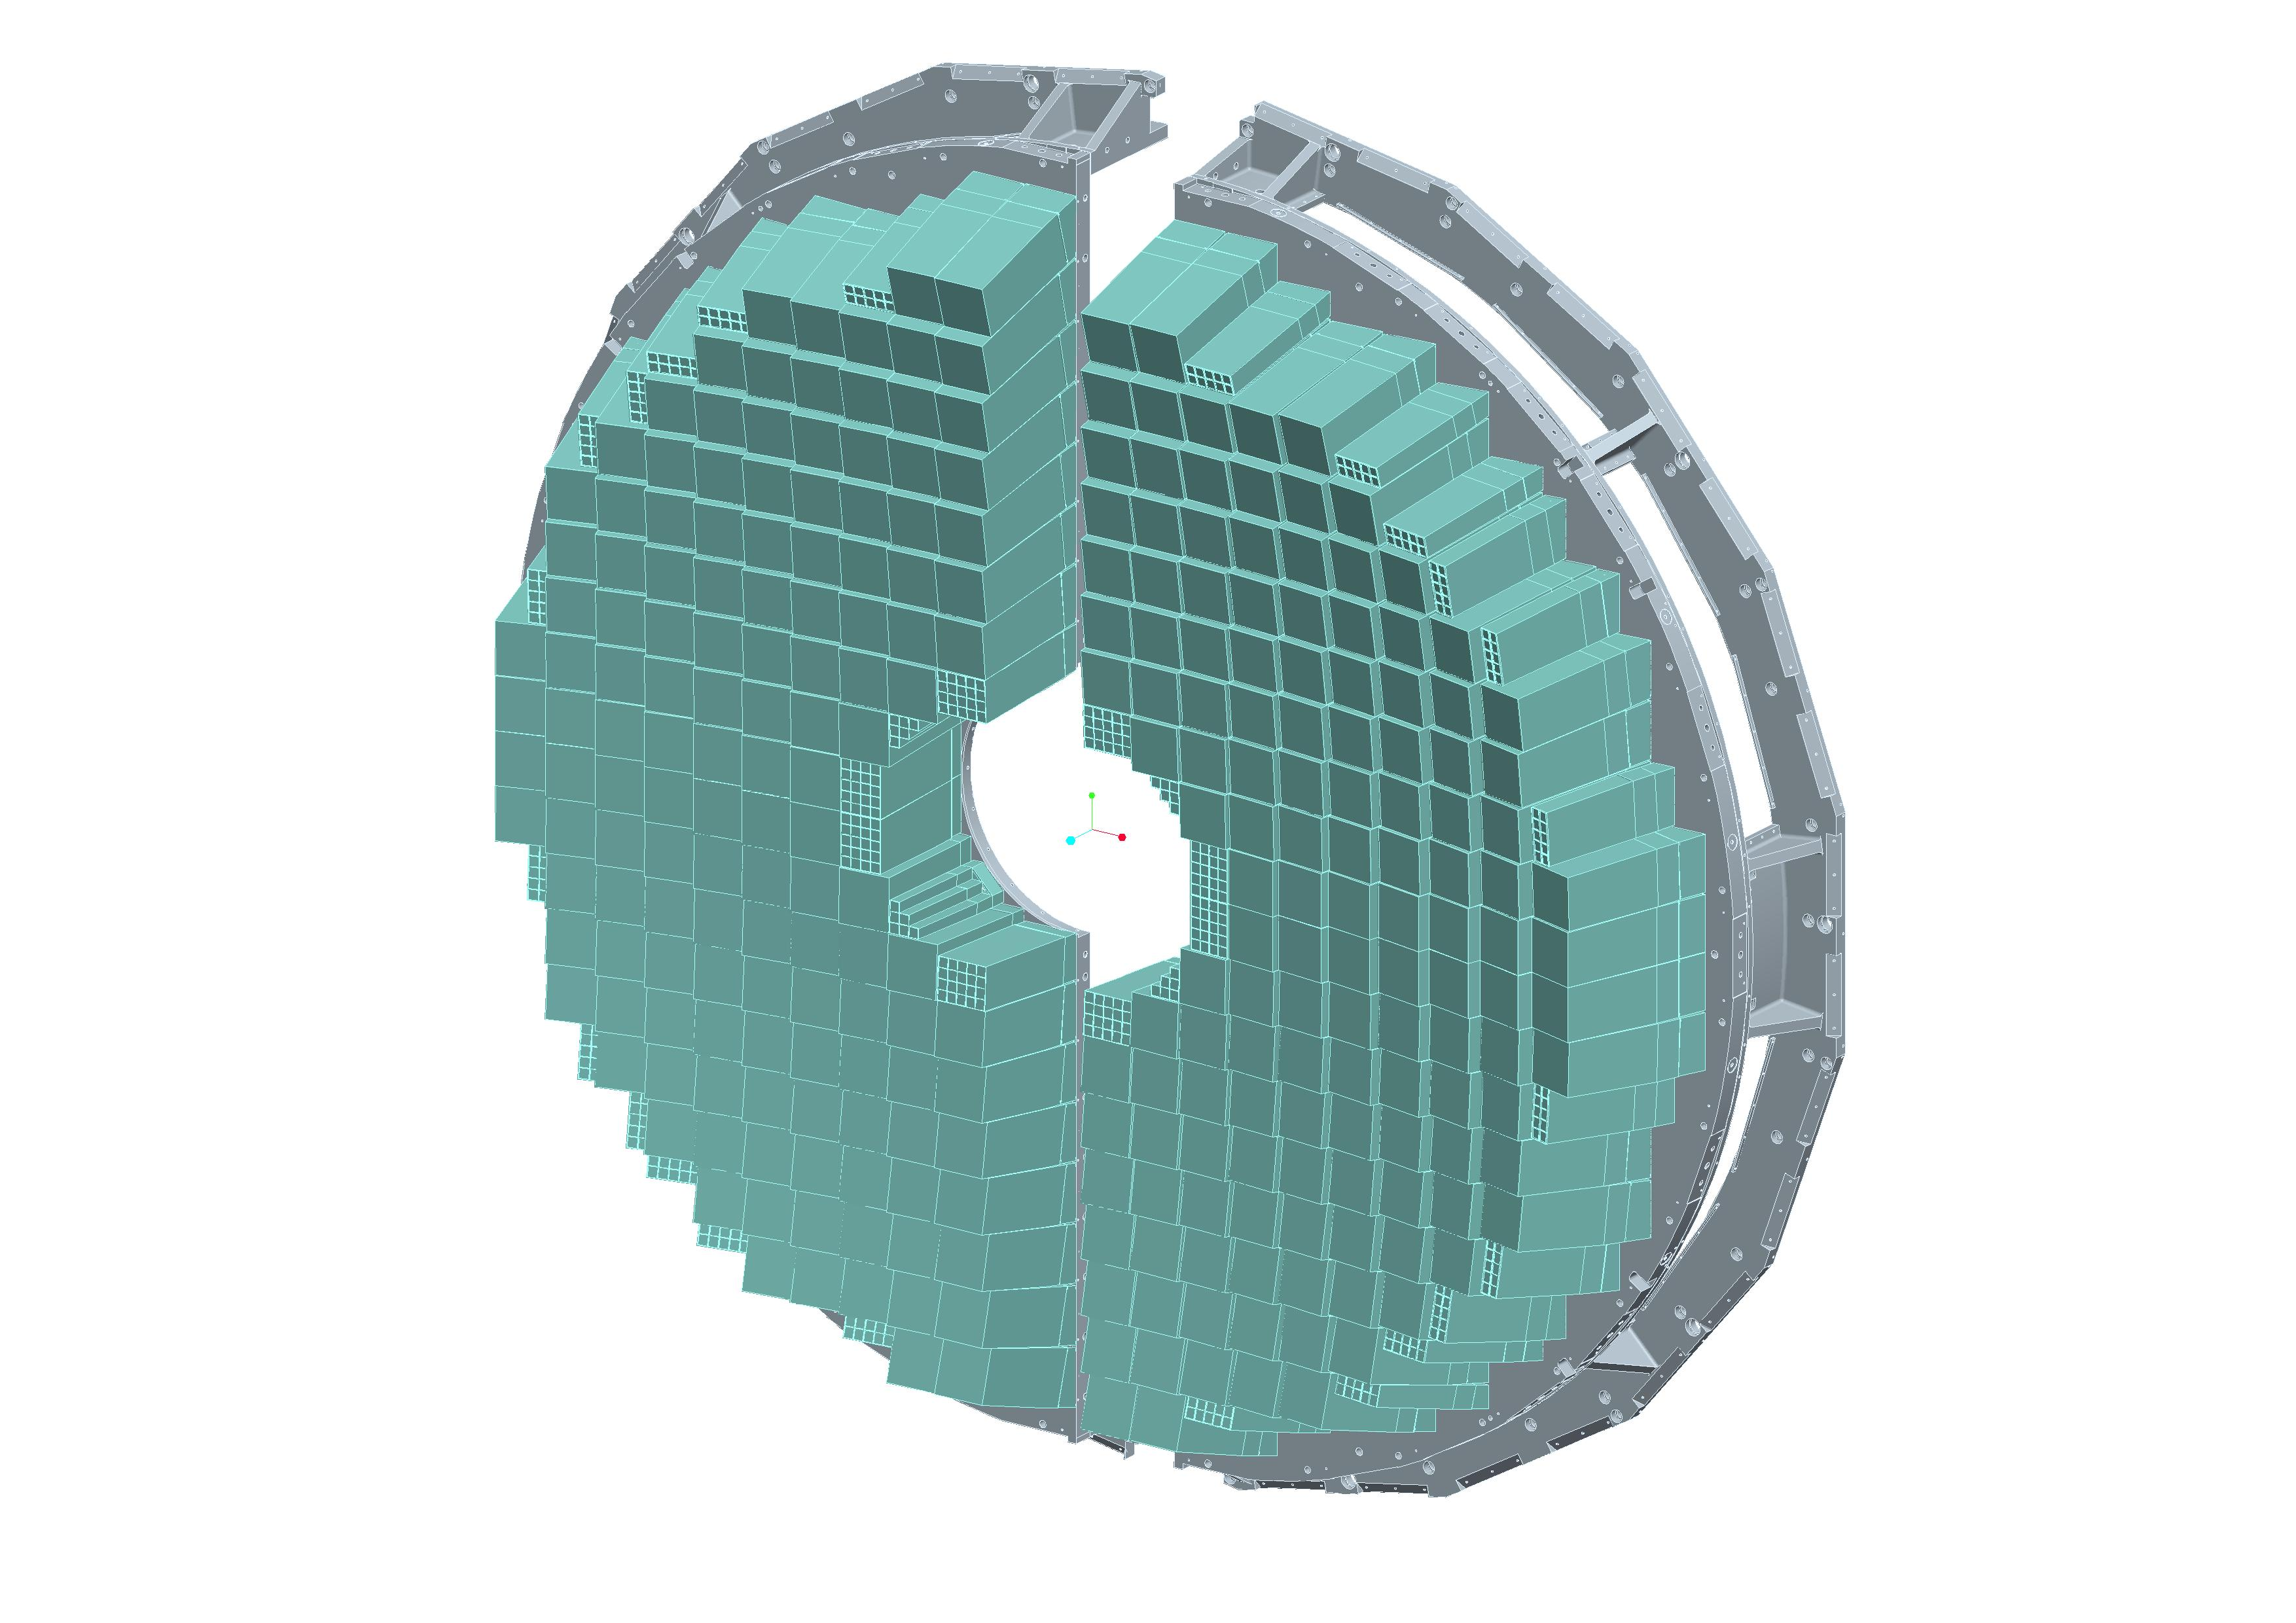
\includegraphics[scale=0.06]{THESISPLOTS/endcap_CMS.png}} 
\captionof{figure}{Deviation of the timing difference as a function of $A_{eff}/\sigma_{n}$ between two crystals sharing an energy in the same electromagnetic shower obtained during electron testbeam measurements. The single crystal energy scales for barrel~(EB) and endcap~(EE) is overlaid. The fitted results give $N = (35.1 \pm 0.2)$~ns and $\bar{C} = (20 \pm 4)$ ~ns. }
\label{fig:FitTimeRes}
\end{center}
A timing resolution better than $100$~ps for energy values $A_{eff}/\sigma_{n}$ greater than $400$~ADC counts is obtained. This demonstrates that for a perfectly calibrated ECAL crystals and energy deposits of $E > 20$~GeV in the barrel, we can obtain a resolution better than $100$~ps. 

%%%%%%%%%%%%%%%%%%%%%%%%%%%%%%%%%%%%%%%%%%%%%%%%%
\subsection{Timing Calibration Procedure}
%%%%%%%%%%%%%%%%%%%%%%%%%%%%%%%%%%%%%%%%%%%%%%%%%%%%%
Timing calibration is performed such that photons traveling along a straight path with speed close to the speed of light, $\beta \approx 1$, produced from proton-proton collisions at IP will arrive at the surface of ECAL crystals  with an average time of $0$~ns. This means, photons or electrons arriving at an ECAL crystal with significantly and positively large arrival time, have either been produced from massive particles traveling with very small velocity~(slow moving particles, $\beta << 1$) or were produced from a decay point and traveled a path which significantly deviates from the obvious straight path connecting the IP to the crystal.
Large arrival time photons or electrons could also be produced in the decay of temporarily stopped particles inside the CMS detector. To reduce contributions from photons with mis-reconstructed or mis-measurement time, we time calibrate all the 75848 ECAL \pb crystals.
Timing calibration also ensures the synchronization of all the component objects of a given event and assigns that event to the correct LHC proton-proton collision or bunch crossing.
The presence of the "$T_{MAX}$ Phase", the difference in pulse shape between each crystal, variation in time of flight by a few nanosecond~(ns) and the different intrinsic delays among channels allow for timing calibration at two separate levels.
At the level of the front end electronics ~(FE) consisting of $5\times5$ crystals, one is capable of performing an initial internal timing synchronization by adjusting in steps of 1.04~ns among these crystals. Determining the values of adjustments to be made is referred to as \textit{Hardware Synchronization}. Offline, during event reconstruction, we can find and assign timing constants such that the measured crystal time for photon objects is on average zero for true collision events arriving in a straight path from IP.

\subsection{Offline Timing Calibration}
%%%%%%%%%%%%%%%%%%%%%%%%%%%%%%%%%%%%%%%%%%%%%%%%%%%%%%%%%%%%%%%%%%
The purpose of the offline calibration is to provide timing adjustments constants for each channel~(crystal). % such that on average the measured time for that channel is zero.
 These constants are derived from  proton-proton collision data to adjust for global phase shift in timing measurements caused by shifts in the CMS clock relative to the LHC bunch crossings and de-synchronizations introduced during hardware interventions during detector repairs. The global timing shifts caused by CMS clock timing drifts can be about 1~ns while that caused by hardware intervention can be $3$ to $5$~ns. The calibration constants obtained for each crystal are of opposite sign to the average time measured from the reconstructed hits of each crystal.
The calibration procedure begins with identifying  timing shift reported in the CMS or ECAL detector running electronic~(e-Log) book or the CMS or ECAL data acquisition monitoring~(DQM) and followed by using  reconstructed crystal hits or rechits from recently recorded or prompt data to measure the calibration constants for each channel. The validated calibration constants in an XML files are uploaded into the online configuration database with existing hardware settings for reprocessing of CMS full datasets used for physics analysis.
This process is performed throughout the entire LHC proton-proton collision period each year. At the end of each calibration process, the set of calibration constants developed for that period of time is called its \textit{interval of validity}~(IOV). The data used in measuring the timing constants is specified by run range of events signifying a period over which proton-proton collisions occurred. During the entire LHC run period in 2011, a total of 17 IOVs were developed while during 2012 LHC run, a total of 44 IOVs were produced. The raw dataset used in producing the calibration constants consists of mostly superclusters with crystal hits from Level-1 triggered events of loosely triggered  photons, electrons and hadrons with large electromagnetic contributions. Datasets with such events are called \textit{ElectronHad} or \textit{PhotonHad}. Rechits from these events must pass a selection criteria which include, the event time~(an average over it's rechits) must be smaller than 5~ns, rechits must belong to a basic cluster whose transverse energy is atleast 2~\GeV, the signal amplitude must not be lower than 26(47) or 100~(in LHC 2012) ADC counts~(corresponding to an energy of about 1(3)~GeV ) for rechits in EB(EE), the reconstructed rechit time must be within 5(7)~ns from either side of zero in EB(EE) and to reduce the presence of anomalous crystal hits, the ratio of the sum of energies of the north, south, east and west neighboring crystals excluding the crystal with the highest energy to that of the energy of the highest energy crystal must be greater than 5\%  or equivalently $ 1 - E_{4}/E_{1} < 0.95$~(the \textit{swiss-cross} variable). This swiss-cross variable is very useful for rejecting events with anomalous crystal energy deposits. The selected rechits are used to make a timing distribution for each channel requiring each channel to have at least 10 rechits.
\newline
After extracting the average time per crystal, the reverse of its value measured is the time calibration constants or inter-calibration coefficient used for timing alignment. The variance represents the spread in the measurement of the calibration constant. For channels with less than 10 valid rechits, the average time of all the other channels is assigned to them as their inter-calibration coefficient. We validate these constants obtained by performing a closure test which involves  applying the reversed values of these constants to the same or different set of events and showing that the measured average time over rechits per channel is 0~ns to within the accuracy of the calibration method and small event migration in the event sample. The event migration effects are of the order of 10~ps.
The figures \ref{fig:TimeCalib} show two dimensional distribution maps of the mean time for each crystal for all the 61,200 crystals in EB and 14648 crystals in EE showing the mean time distribution before~(\textit{top 3 plots}) and after~(\textit{bottom 3 plots}) calibration.
Further details of the full IOVs produced for the entire LHC Run 1 can be found here \cite{ECALCAL}.
%%%%%%%%%%%%%%%%%%%%%%%%%%%%%%%%%%%%%%%%%%%%%%%%%%%%%%%%%%%%%%%%%
\begin{center}
\centering
\mbox{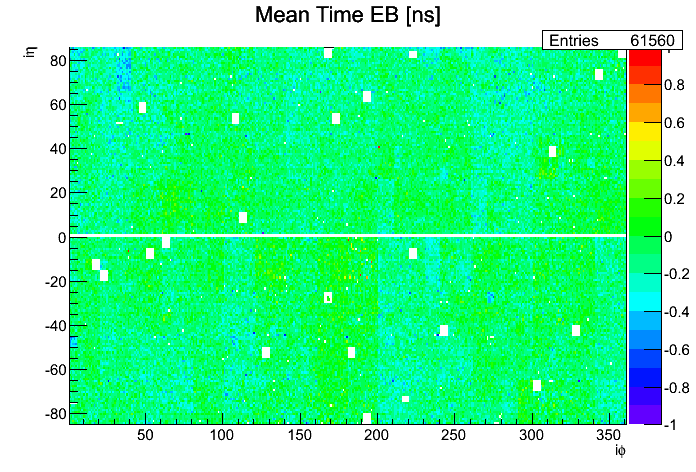
\includegraphics[height=0.40\textwidth, width=0.80\textwidth]{THESISPLOTS/calibDiffMapEB_Before_Calibration.png}}
\mbox{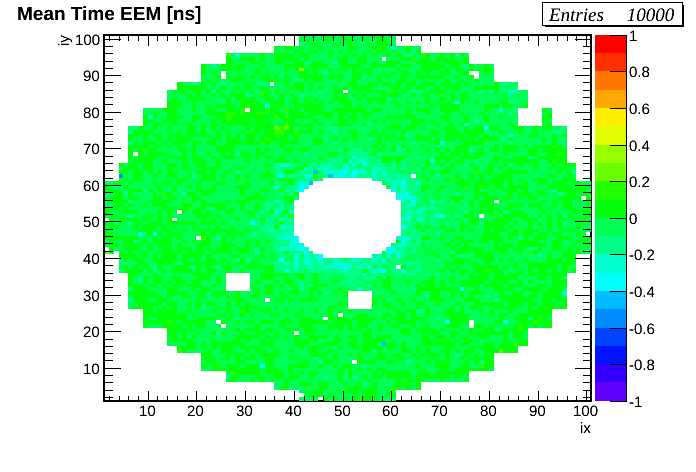
\includegraphics[height=0.42\textwidth, width=0.45\textwidth]{THESISPLOTS/calibDiffMapEEM_Before_CALIB.png} \quad
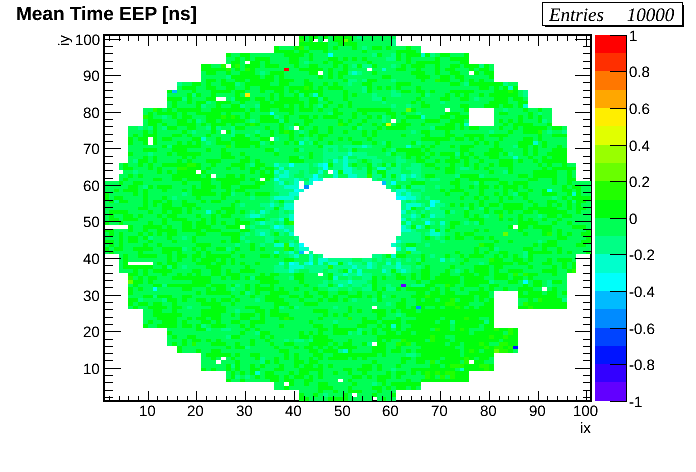
\includegraphics[height=0.42\textwidth, width=0.45\textwidth]{THESISPLOTS/calibDiffMapEEP_Before_CALIB.png}
}
\vspace{1.5cm}

\mbox{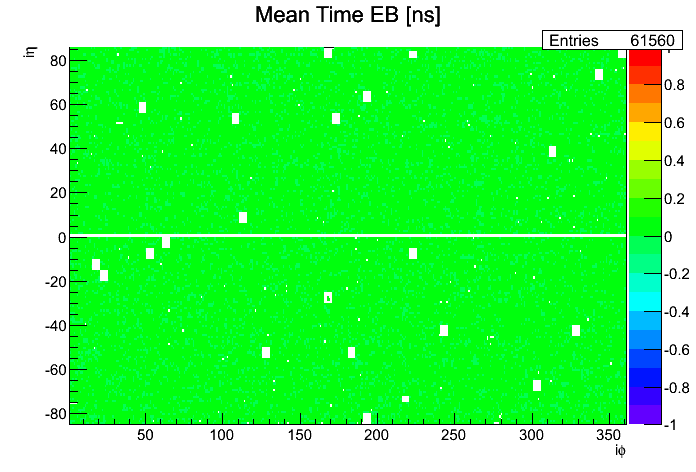
\includegraphics[height=0.40\textwidth, width=0.80\textwidth]{THESISPLOTS/calibDiffMapEB_After_Calibration.png}}
\mbox{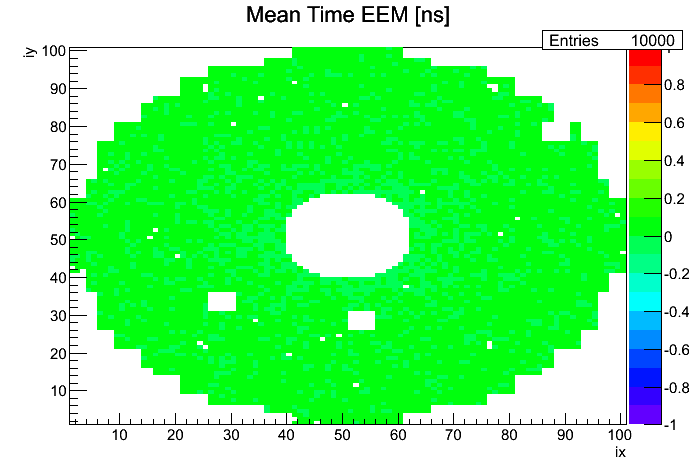
\includegraphics[height=0.42\textwidth, width=0.45\textwidth]{THESISPLOTS/calibDiffMapEEM_AFter_CALIB.png} \quad
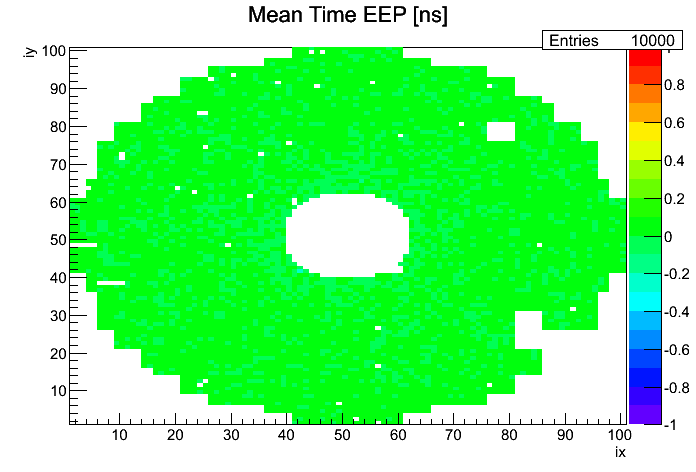
\includegraphics[height=0.42\textwidth, width=0.45\textwidth]{THESISPLOTS/calibDiffMapEEP_After_CALIB.png}
}
\captionof{figure}{\textit{Top 3}: Timing calibration maps showing the distribution of mean time for each channel/\pb crystal in EB~(top) and EE~(below: EE\texttt{-}(left), EE\texttt{+}(right)) before calibration.
\textit{Bottom 3}: Timing calibration maps showing the distribution of mean time after calibration. 
After calibration most crystals have an average time of zero(\textcolor{green}{Green}).}
\label{fig:TimeCalib}
\end{center}

\subsection{Hardware Timing Calibration}
%%%%%%%%%%%%%%%%%%%%%%%%%%%%%%%%%%%%%%%%%%%%%%%%%%%%%%%%%%%%%%%%%%%
It is well known that timing offsets can be introduced during hardware repairs of ECAL front end electronics. These timing offsets are not easily adjustable during offline reconstruction as our method of offline timing calibration simply adjusts for the timing latency settings of the front end electronics using the online database. Hardware settings for readout electronics with timing offsets not properly aligned or calibrated can contribute to worsening of the timing resolution. The traditional method of correcting for this hardware timing offsets or latency during LHC stable proton beam collision has been, in cases of an observed timing offset is to record enough data with the maladjusted hardware settings with timing offset, stop the entire CMS data taking process while LHC proton collisions are still ongoing, use the collected data to extract the hardware timing offsets, use these extracted timing offsets to adjust the hardware settings and finally continue with recording data with the CMS detector. These timing offsets are spotted and extracted during Data Quality Monitoring~(DQM) and data certification hardware readout electronics performance routines. Although this method is reliable, it encourages long and intermittent data recording downtime as stopping the ECAL section of the CMS detector in order to adjust the settings of the hardware readout electronics leads to lost in data recording time which in some cases if the reason for reduced luminosity recorded by CMS compared to luminosity delivered by the LHC during LHC stable proton beams. To reduce this lost, we need an alternative method of adjusting the hardware timing offsets while reducing CMS data recording downtime. 
Our alternative approach to investigating and adjusting the hardware latency settings for timing offsets after the CMS or LHC machine maintenance intervention during technical stop or machine development was to use laser data instead of proton-proton collision data for performing timing adjustment. ECAL uses lasers to study and adjust for depreciated crystal energy resolution caused by loss in crystal transparency due to radiation. 
\newline
The ECAL laser system comprise of two lasers, a 440~nm wavelength~(close to peak emission for \pb crystals) laser for monitoring crystal transparency lose and a 796~nm wavelength laser for monitoring readout electronics chain from APDs to ADCs. Both lasers have jitter of less than 4~ns every 24 hours run. To account for this jittery effect, the timing from the laser is averaged over 600 event pulses. The time for each crystal from laser is expected to be the same as the time from data and is represented as $\mathbf{T^{APD}_{MAX}}$. The ECAL laser system is also equipped with a fast acquisition card called MATACQ. The time for each channel recorded using the Matacq is also averaged over 600 event pulse denoted as $ T_{Matacq}$.
The difference in $ T^{APD}_{MAX} - T_{Matacq} $ between these two times averaged over the  25 crystals in a Clock and Control Unit ~(CCU) gives the time for each CCU, $ t_{CCU} = \left\langle T^{APD}_{MAX} - T_{Matacq} \right\rangle $. In order to calculate the timing shift of 25 crystals belonging to the same Front End~(FE) electronics, we monitor for any changes to this average value before~($t^{B}_{CCU} $) and after~($t^{A}_{CCU} $) hardware intervention during detector maintenance.  The difference, $\Delta t_{CCU} = t^{A}_{CCU} - t^{B}_{CCU}$, after correcting for any global shift, and averaged over all the 25 crystals, \ie ~$\left\langle t^{A}_{CCU} - t^{B}_{CCU} \right\rangle $, gives the timing shift and calibration constant for that CCU and is done the same way for all the 68 CCUs in a given supermodule~(SM) or front end detector~(FED). Any global timing shift of all the crystals in a given FED is due to the laser light distribution in-homogeneity or evolution of the laser pulse due to different optical fiber supply of laser light to each CCU. Each FED or SM has 1,700 \pb crystals. 
The plots in figure \ref{fig:TimeLaser} show our current observation status after monitoring for any shift in time within each CCU using laser. It shows the distribution of the CCU timing difference, $\Delta t_{CCU}$ with its root mean squared~(RMS) value for each CCU before and after machine intervention. Considering the subtraction of the global shift per FED also reduces the possibility of false timing shift in a given CCU.
Using the average time subtraction method with laser data, we are able to measure each CCU timing shift to within 0.2~(0.5)~ ns EB~(EE) in precision. This tool and procedure allow for adjusting the hardware timing settings during CMS data  recording without the need for collision data. However some validation studies for this method is yet to be performed.  
In summary, we use crystal time from laser data to measure possible hardware timing offsets and use these timing offsets to provide new hardware settings prior to proton-proton collision. This adjustment can be performed online or \textit{in-situ} by using the ECAL readout electronics condition database system. The full procedure including technical details for performing hardware latency adjustments online using collision data or laser data is well described in \cite{ECALHW}.
\clearpage
\begin{center}
\centering
\mbox{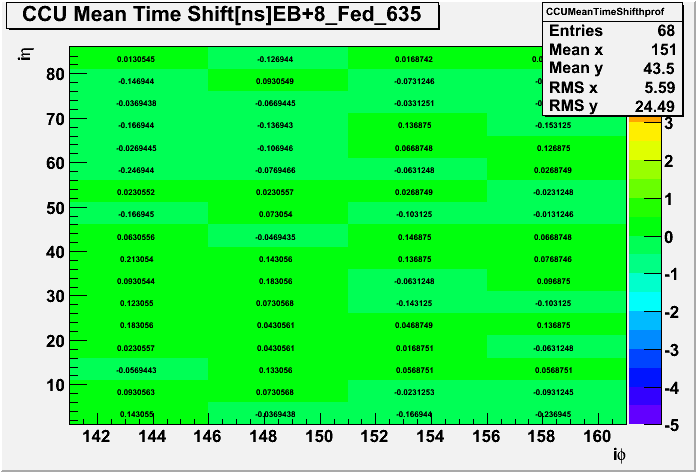
\includegraphics[height=0.45\textwidth, width=0.45\textwidth]{THESISPLOTS/CCU_Mean_Time_ShiftEB_Plus8_Fed_635.png} \quad
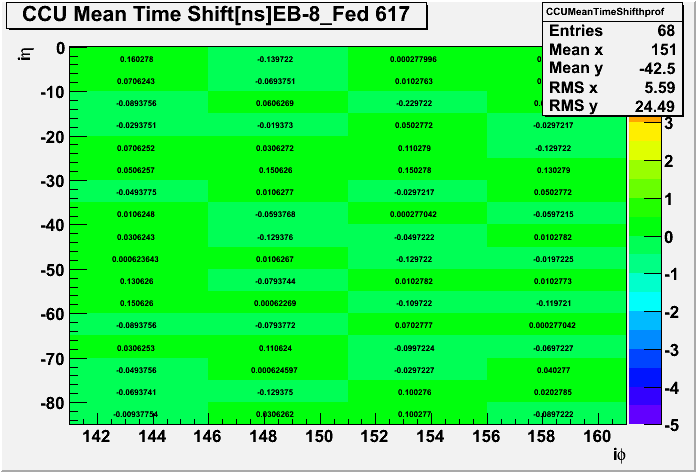
\includegraphics[height=0.45\textwidth, width=0.45\textwidth]{THESISPLOTS/CCU-Mean-Time-Shift-EBMinus8-Fed617.png}}

\vspace{1cm}
\mbox{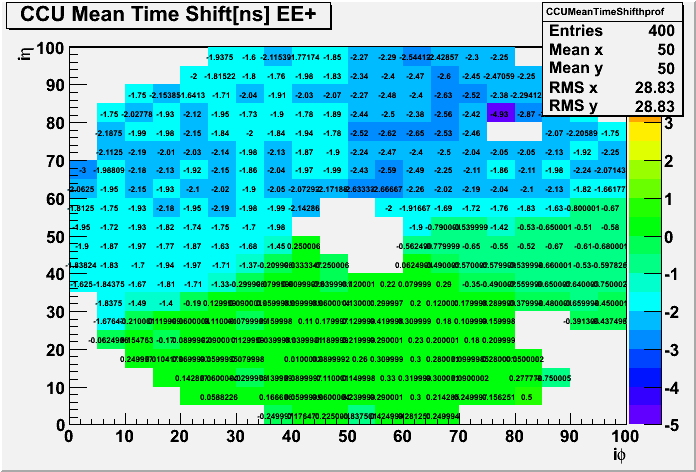
\includegraphics[height=0.45\textwidth, width=0.45\textwidth]{THESISPLOTS/CCU_Mean_Time_Shift_EEP_Laser.png} \quad 
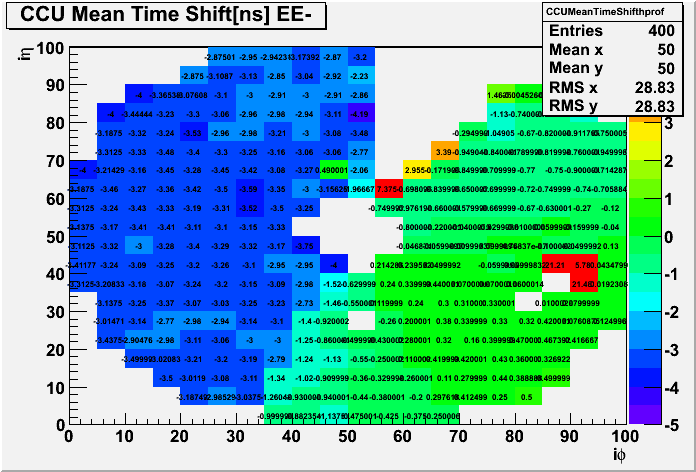
\includegraphics[height=0.45\textwidth, width=0.45\textwidth]{THESISPLOTS/CCU_Mean_Time_Shift_EEM_Laser.png}}
%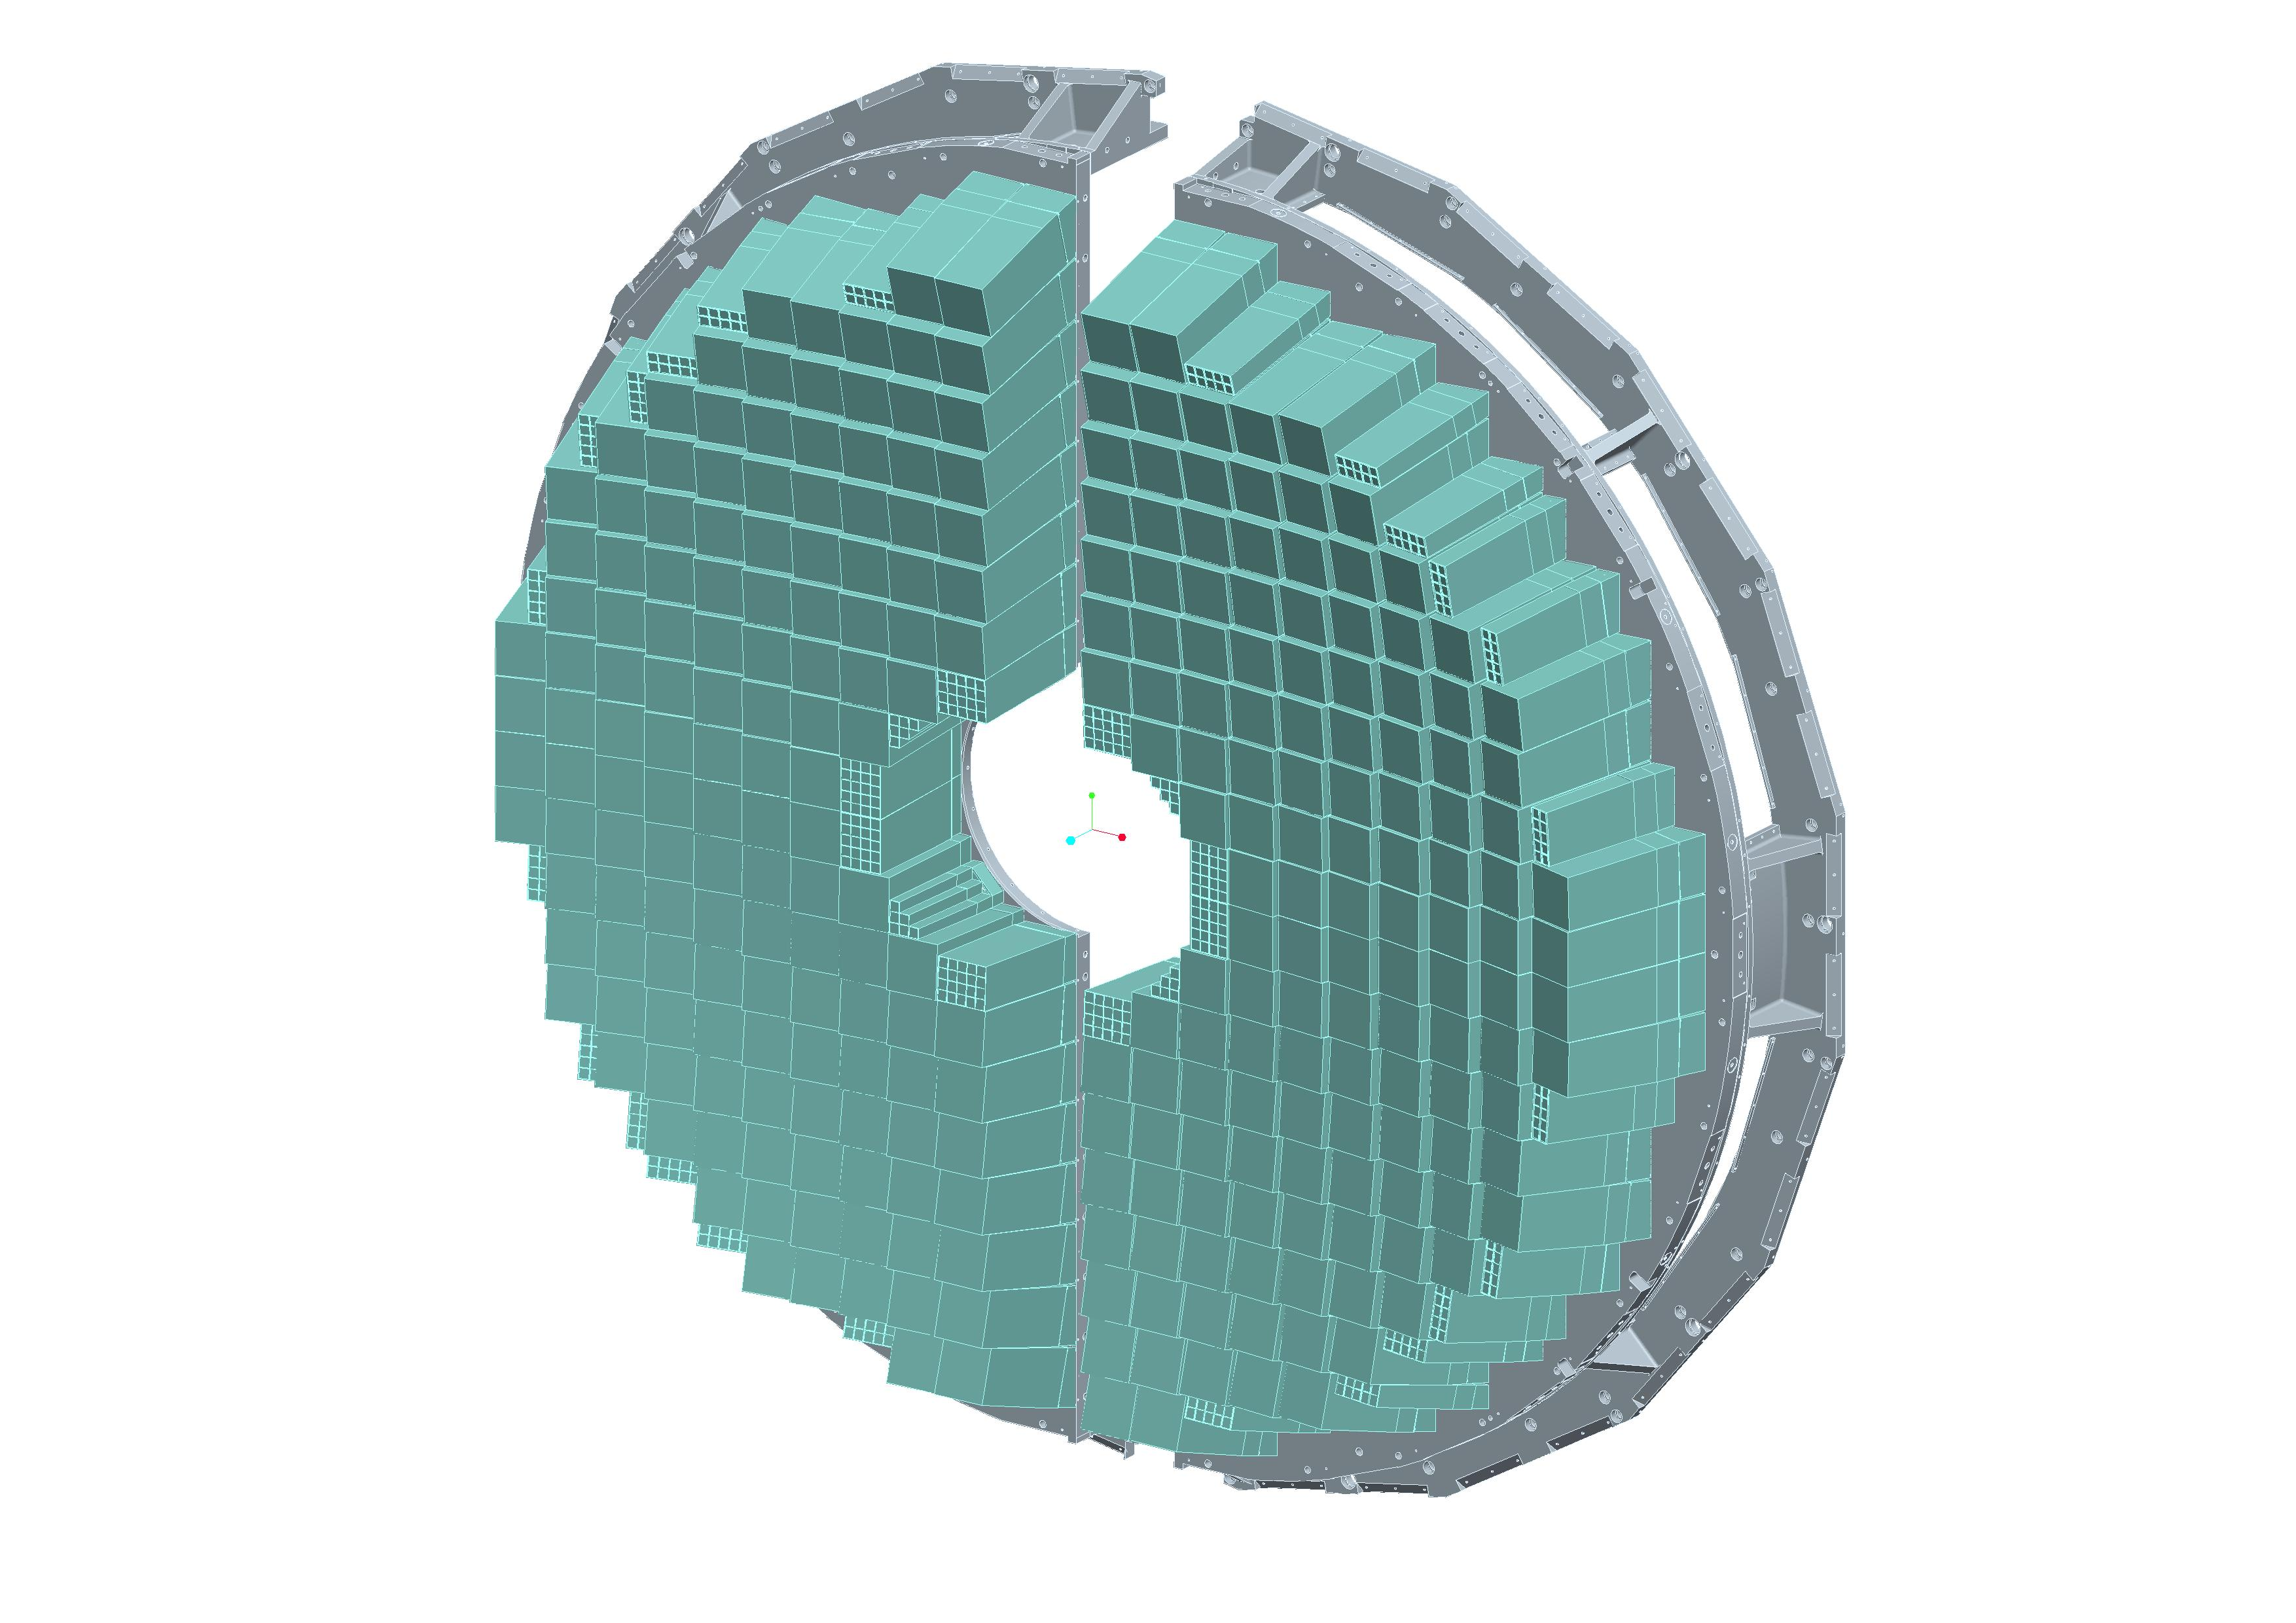
\includegraphics[scale=0.06]{THESISPLOTS/endcap_CMS.png}} 
\captionof{figure}{\textit{Top}: Crystal mean time distribution for crystals in readout electronics EB$\pm$8. Crystal time obtained from Laser data.
\textit{Bottom}: Clock and Control Unit ~(CCU) mean timing shift distribution of readout electronics of EE$+$ and EE$-$. The adjustment for global timing shift per FED due to difference in light source for each CCU has been shown to reduce the possibility of CCU showing false timing shift. The figures show $\Delta t_{CCU}$ distributions after the global shift has been removed. }
\label{fig:TimeLaser}
\end{center}
%%%%%%%%%%%%%%%%%%%%%%%%%%%%%%%%%%%%%%%%%%%%%%%%%%%%%%%%%%%%%%%%%%
\subsection{Timing Bias}
%%%%%%%%%%%%%%%%%%%%%%%%%%%%%%%%%%%%%%%%%%%%%%%%%%%%%%%%%%%%%%%%%%
The ratio algorithm described in Section $4.2$ for extracting the amplitude and time of an event signal from ten digitized samples of a crystal or channel is assumed to perform efficiently well for all energies of the hits. However, during LHC Run 1 proton-proton collision, it has been observed that this is not the case, especially for very energetic particles. An inherent timing bias is introduced by the MGPA for incoming electromagnetic particles with energy above the gain transition point. The energy  deposited by an incoming particle on a crystal is recorded as an ADC count, $A$, which is the signal amplitude of the recorded pulse shape. This ADC count can be converted into energy in \GeV through some conversion factors and adjustments. The full conversion from ADC counts to \GeV of a crystal energy is expressed using equation \ref{eq:AMP2GeV}.
\begin{equation}{\label{eq:AMP2GeV}}
    E_{i} =  G \cdot S_{i}(t) \cdot C_{i} \cdot A_{i} 
\end{equation}
Where $G$ is an ADC-to-GeV conversion factor equal to $0.039$($0.063$) in EB(EE). $C_{i}$ is the inter-calibration coefficients accounting for individual channel response and $S_{i}(t)$ is the correction term (usually from laser data) accounting for radiation-induced channel response.  $S_{i}$ changes over time. The Gain~1 transition point is at $4096$~ADC counts corresponding to $159.744$~\GeV in EB and $258.048$~\GeV in EE. The subsequent Gain~6 and 12 transitions are at energy values of \TeV energy level.
The bias in timing introduced by these gain transitions cannot be calibrated at hardware, so we developed a method of adjusting the
timing measurements for the timing bias at the CMS event reconstruction level.
Using reconstructed hits with similar selection as our offline timing calibration, selected hits are also required to be part of a basic cluster~(usually $3\times 3 $ or $5\times 5$ matrix of crystals). These hits must have amplitude with channel noise consideration above $10$ ADC counts. We reject hits with very large timing biased and large swiss-cross variable beyond our selection threshold~(0.99). A distribution of the hit time against its amplitude is plotted and then sliced in bins of amplitude. Bins containing at least 7 hits are fitted using a Gaussian function constrained within $\pm 7$~ns. The average(mean) and standard deviation(RMS) from these distributions is plotted against their corresponding amplitude or energy to give a distribution of mean and standard deviation  against amplitude. This procedure is performed for different \textit{Modules} or pseudo-rapidity~($\eta$) range starting from $\eta = 0$ which is \textit{Module}~1 in barrel to $\eta = 3$ for high-eta in endcap.
Figure \ref{fig:TimeBias} shows the mean against energy distribution for different reconstruction CMS Software~(CMSSW) release versions where these timing bias corrections have been applied~(CMSSW5XY) and have not been applied~(CMSSW44X) during object reconstruction. 
%It is now a standard procedure in CMS that these timing biases are applied for all CMS releases. %All CMSSW releases beyond CMSSW5XY now have these bias corrections applied. 
%The dataset used for this reconstruction is the \textit{DoubleElectron} and \textit{Photon} dataset processed using CMSSW44X release during LHC RUN 1 and later reprocessed using CMSSW53X with the bias corrections applied. 
\begin{center}
\centering
\mbox{
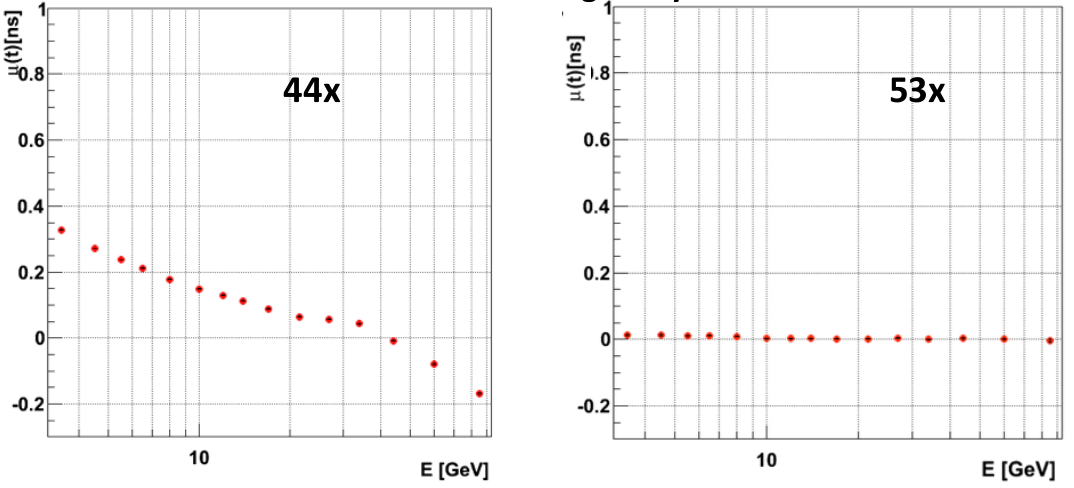
\includegraphics[height=0.450\textwidth, width=0.85\textwidth]{THESISPLOTS/AmplitudeVsTimeCMSSW_Comparison.png} } 
\vspace{5cm}
\mbox{
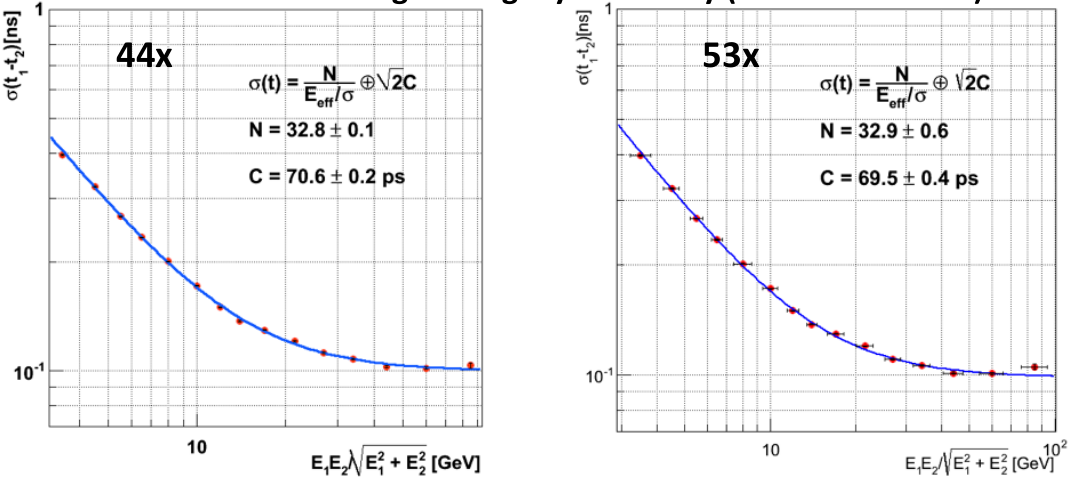
\includegraphics[height=0.460\textwidth, width=0.85\textwidth]{THESISPLOTS/TimingResolutionCMSSW_Comparison.png}
}
\vspace{-5cm}
\captionof{figure}{Distribution of mean time~($\mu$),\textit{top row}) and timing deviation~($\sigma$, \textit{bottom row}) as a function of crystal energy for EB prior~(left) and after~(right) timing bias corrections depending on amplitude have been applied.}
\label{fig:TimeBias}
\end{center}

We investigated for dependence of the timing measurements on the crystal position in ECAL from $\eta = 0$ to $\eta = 3.142$. The results in figure \ref{fig:EtaDep} show no crystal position or $\eta$ dependence.
% and over time, which in the this case we use the proton-proton collision run period~(RUN Number)
There are other timing biases of the order of about 100~ps have been observe in the difference in time for crystals belonging to different electronics. Such timing bias are not yet understood.

%We have also performed detail studies to check for $\eta$ and run dependence contributions to the timing bias. 
%In figure \ref{fig:EtaDep}, we show the distribution of the mean time~($\mu$) and standard deviation~($\sigma$) for different modules in different resgions in barrel and sections in endcap. The timing resolution do not show any dependence on pseudo-rapidity~($\eta$), however 
\begin{center}
\centering
\mbox{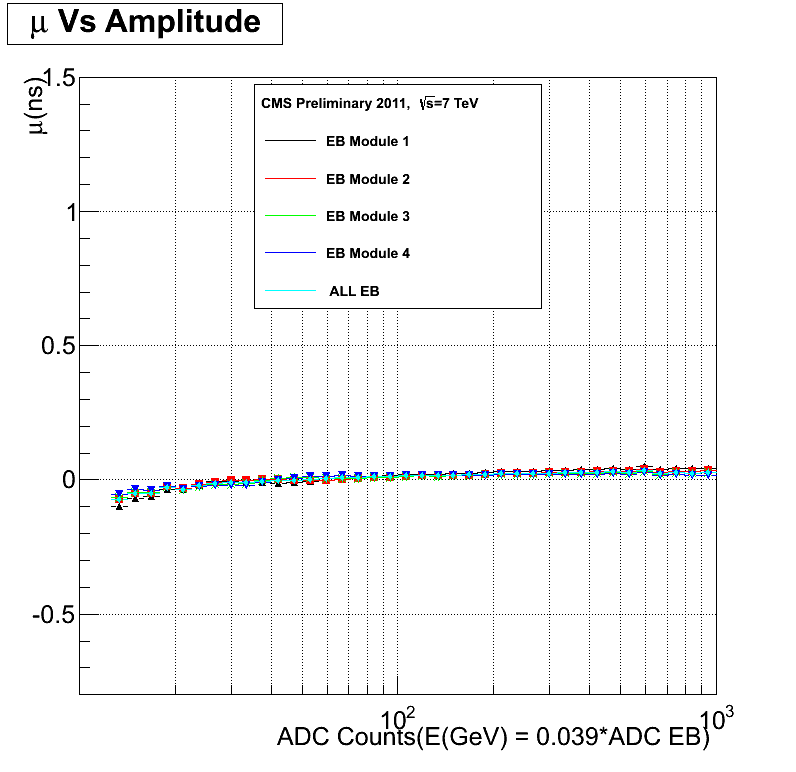
\includegraphics[height=0.45\textwidth, width=0.45\textwidth]{THESISPLOTS/EB_TimeVsAmplitude_StabilityCMSSW_5_3_X.png} \quad
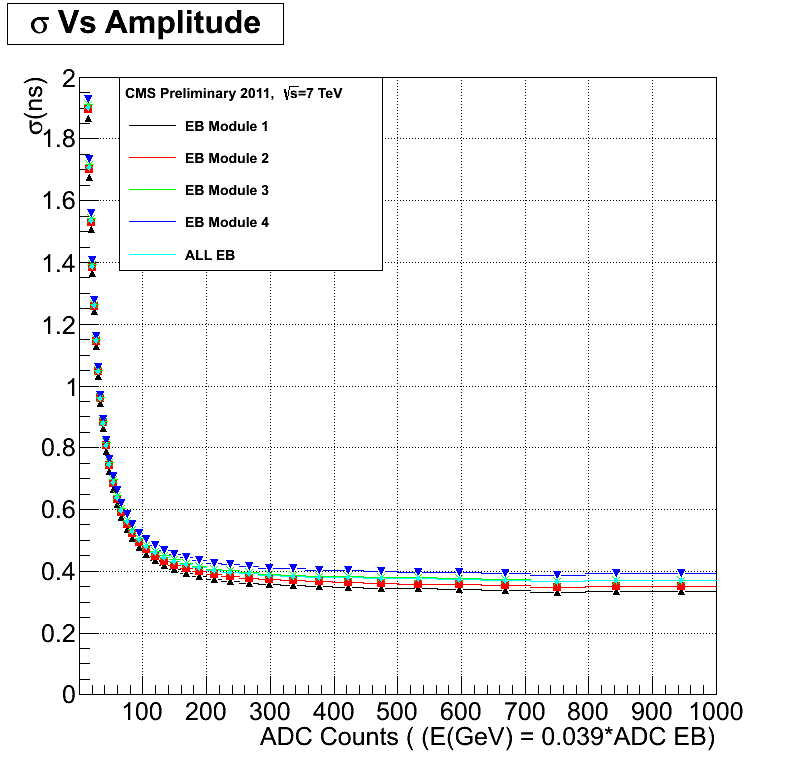
\includegraphics[height=0.45\textwidth, width=0.45\textwidth]{THESISPLOTS/EB_SigmaVsAmplitude_Stability_In_CMSSW_53X.png}}
%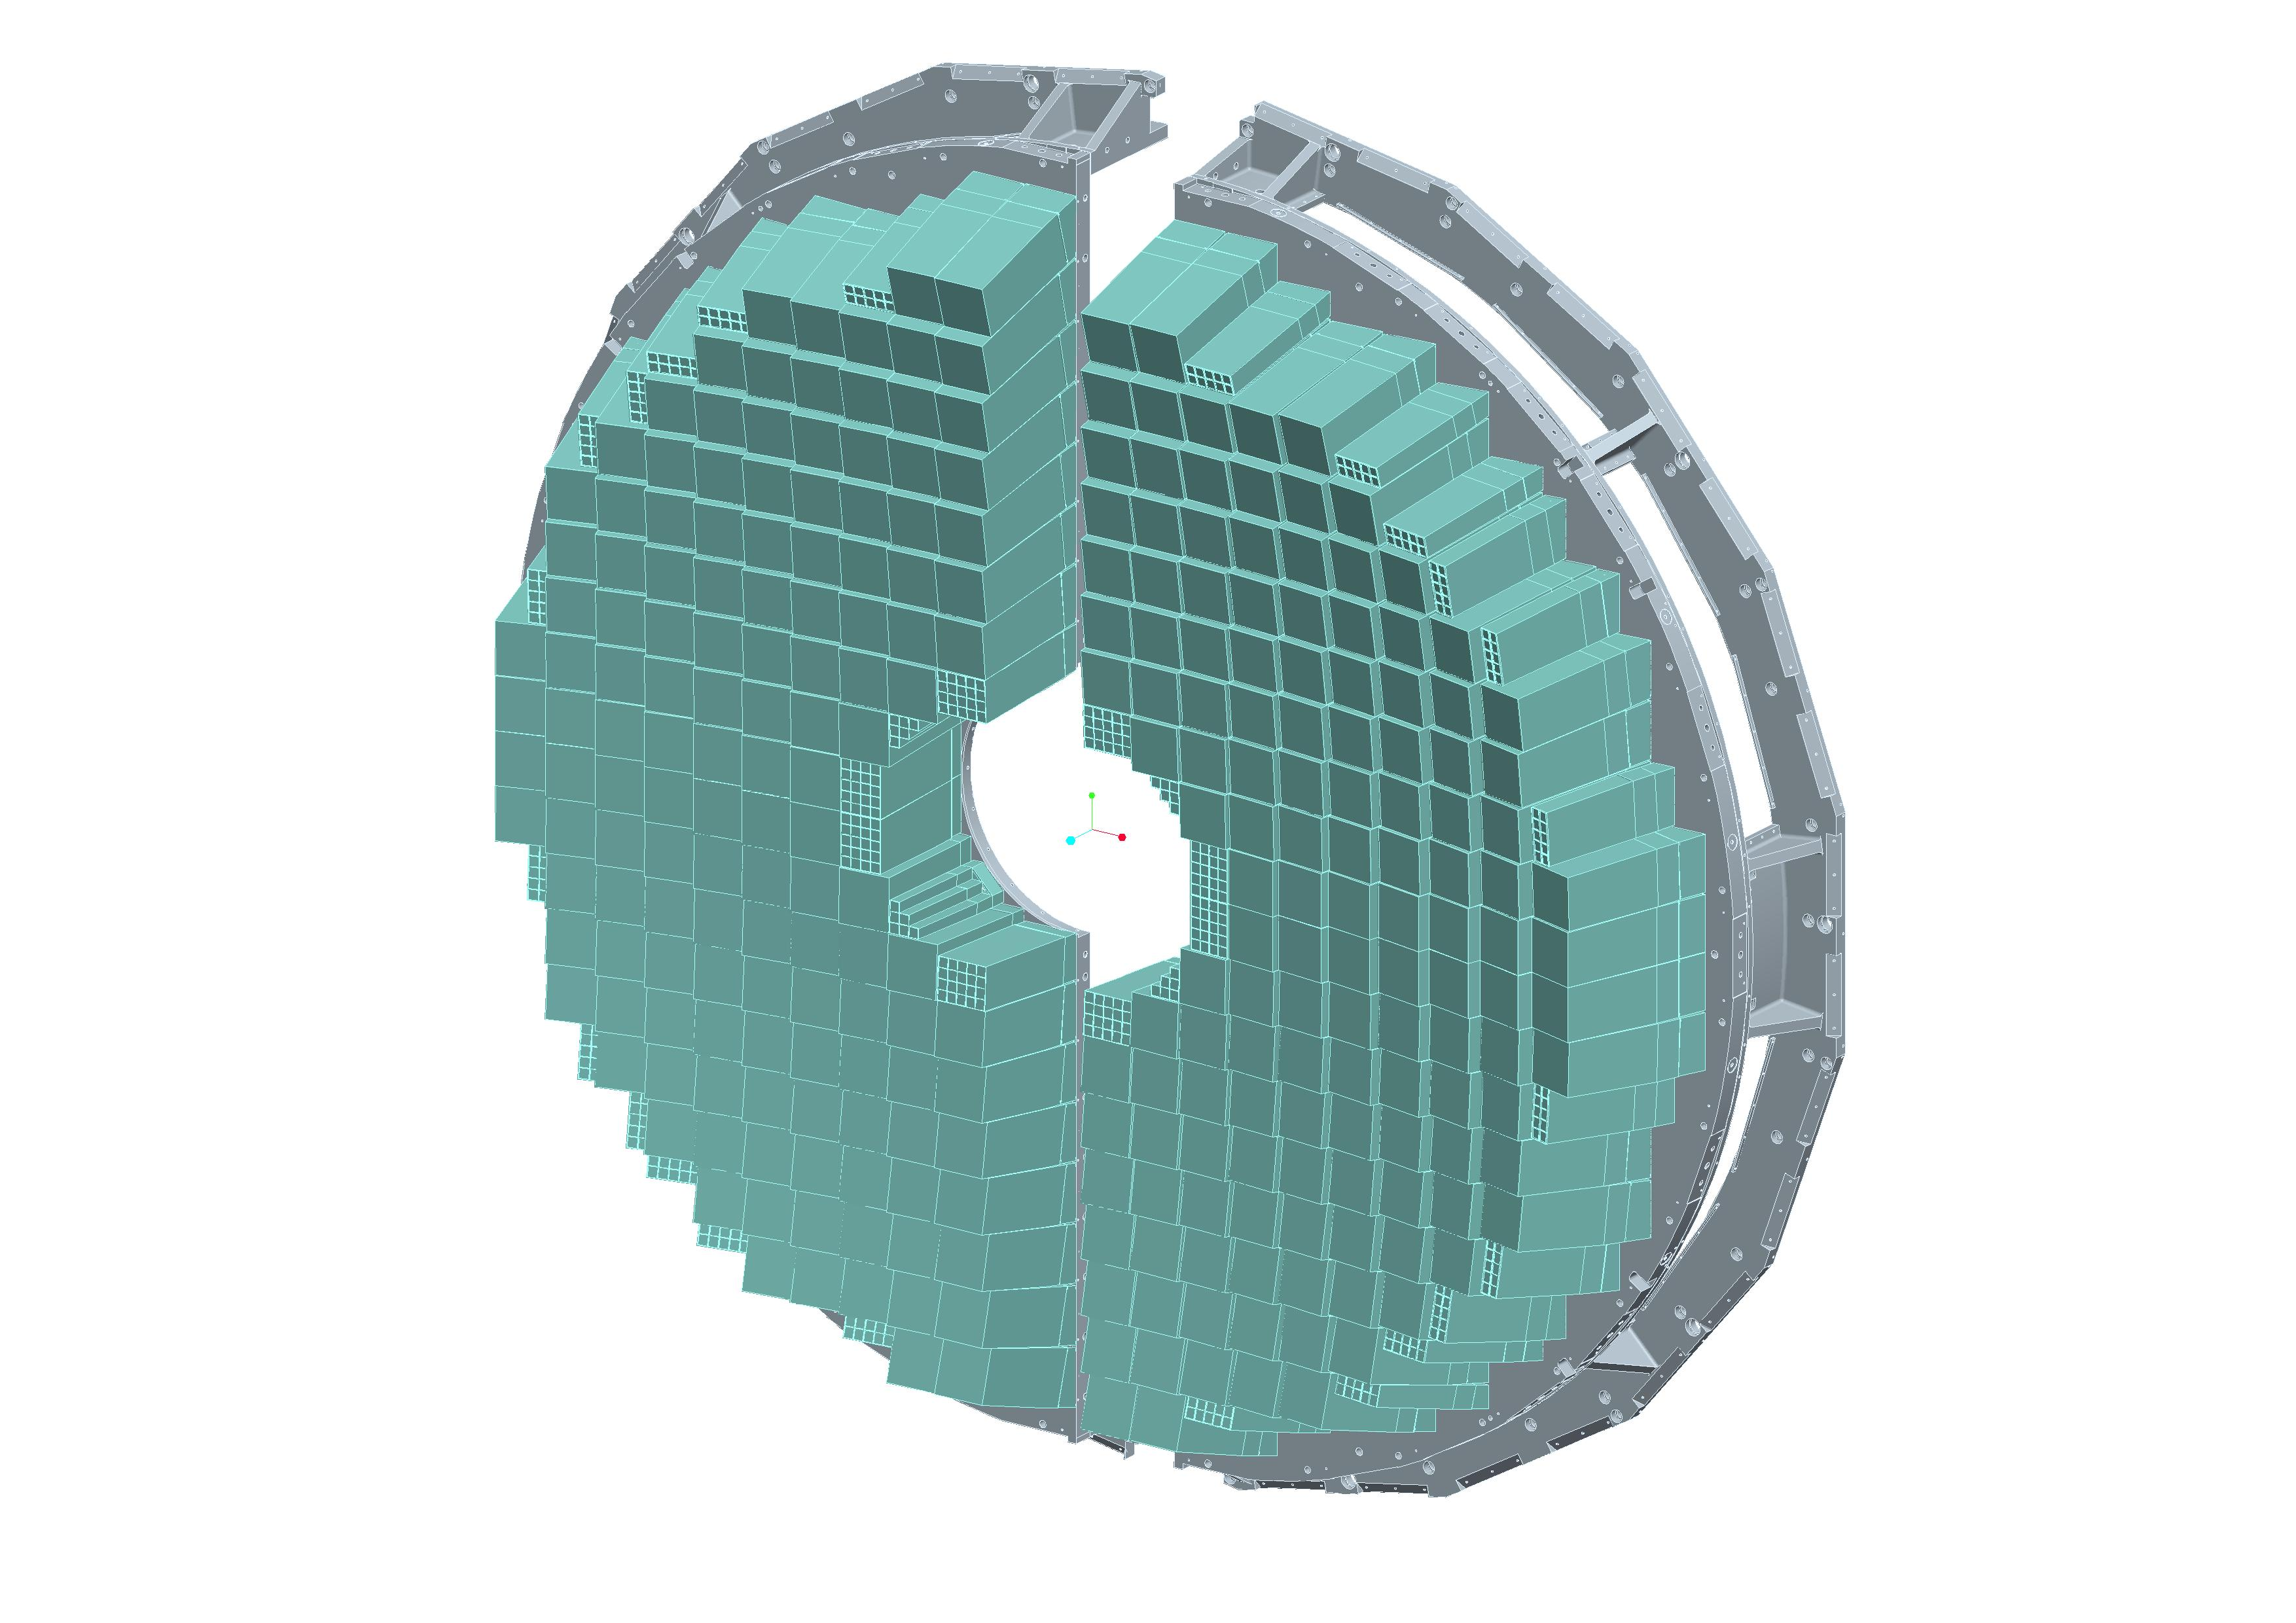
\includegraphics[scale=0.06]{THESISPLOTS/endcap_CMS.png}} 
\vspace{-0.5cm}
\mbox{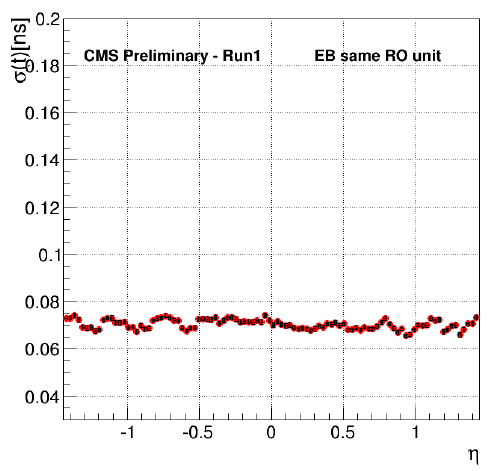
\includegraphics[height=0.50\textwidth, width=0.60\textwidth]{THESISPLOTS/TimeResolution_Vs_Eta.png}}
%\mbox{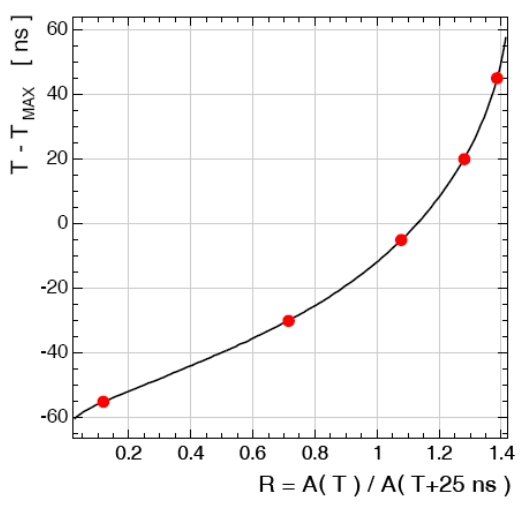
\includegraphics[scale=0.45]{THESISPLOTS/TMaxPhaseVsRatio.png}}
%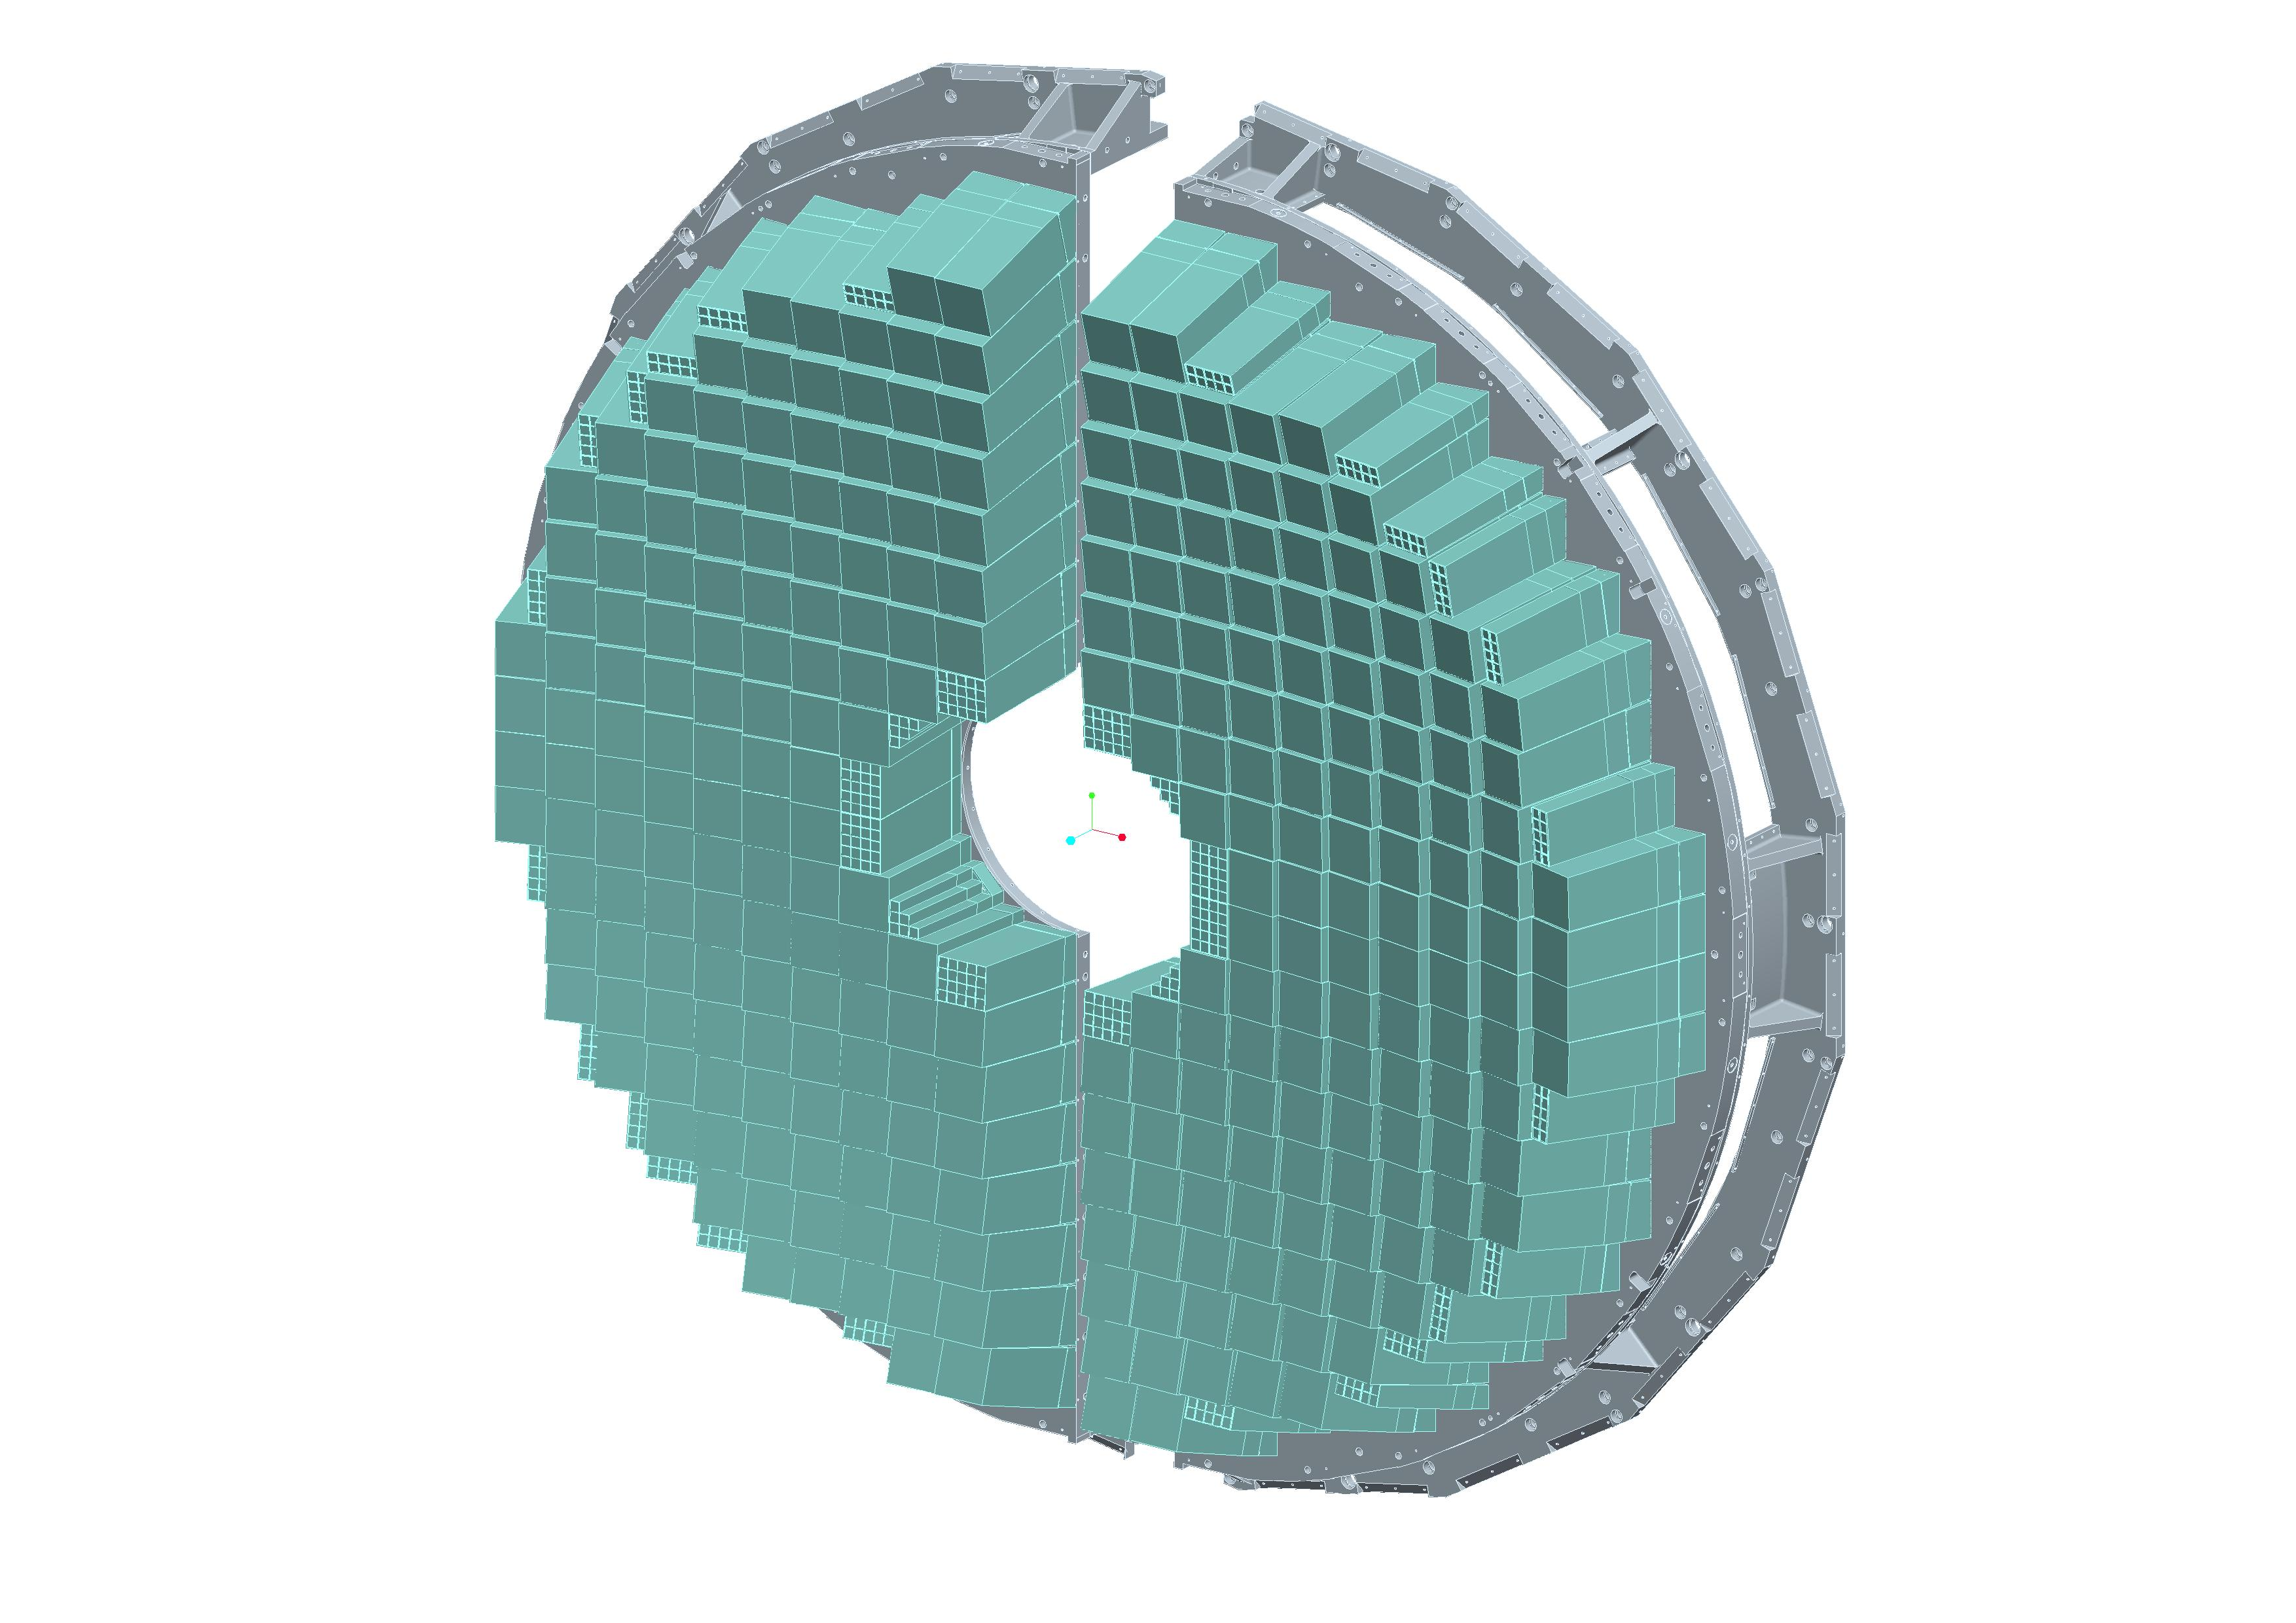
\includegraphics[scale=0.06]{THESISPLOTS/endcap_CMS.png}} 
\captionof{figure}{\textit{Top row}: Distribution of mean time~($\mu$) as a function of amplitude~(left) and resolution~($\sigma$) as a function of amplitude~(right) for different pseudo-rapidity regions in the barrel. ~\textit{Bottom}: All modules in EB combined timing resolution as a function against $\eta$ crystals in the same readout electronics in  barrel~(EB).}
\label{fig:EtaDep}
\end{center}
\clearpage
%%%%%%%%%%%%%%%%%%%%%%%%%%%%%%%%%%%%%%%%%%%%%%%%%%%%%%%%%%%%%%%%%%
%%%%%%%%%%%%%%%%%%%%%%%%%%%%%%%%%%%%%%%%%%%%%%%%%%%%%%%%%%%%%%%%%%
\section{Electromagnetic Calorimeter Timing Performance}
%%%%%%%%%%%%%%%%%%%%%%%%%%%%%%%%%%%%%%%%%%%%%%%%%%%%%%%%%%%%%%%%%%
%Timing calibration is performed to properly align the time of an incoming event which can be misaligned because of poor inter-calibration between different front end electronics, biased on timing due to timing dependence on energy, reduction in \pb crystal transparency due to radiation, hardware intervention during machine repairs and other effects. To measured 
We study the performance of timing measurements by ECAL crystals using well studied physics processes like the decay of a $\PZ$ boson to an electron pair, \ie $\PZ \rightarrow \Pelectron \Ppositron$. 
We use the difference in the arrival time of both electrons at ECAL crystals, which in principle
should be zero, to evaluate ECAL timing measurement performance. This performance is expressed by using the standard deviation, $\sigma_{eff}$, of the difference in arrival time of both electrons.
%The decay of a $\PZ$ boson is well understood and effects due to poor event reconstruction or detector effects are well measured. 
%The idea is to use the two electrons which in principle should have the equal arrival time  and use their measured time difference to estimated the timing resolution performance of the \pb crystals in ECAL. In order to understand different source of poor timing measurements, we study the following different methods for measuring the time of the two electrons:
The crystal arrival time for each electron is the time of the seed crystal~($t_{seed}$) of the electron energy super cluster. The difference in the seed time between
both electrons after correcting for contributions from the bending of the electron travel path inside a strong CMS magnetic field of 3.8~T, $t_{electron1} - t_{electron2} = t_{seed1}-t_{seed2}$, gives a good estimate of the timing resolution performance of the ECAL crystals.
Figure \ref{fig:ZeeTimePerformance2} shows time difference of both electrons adjusted for time of flight corrections while 
figure \ref{fig:ZeeTimePerformance1}, shows the time resolution obtained form the time distrobution of the seed crystal time without correcting for the bending of the flight path contributions.
% using the time of the seed crystal~(crystal with highest energy) in the electron suspercluster and
%\begin{enumerate}
%\item The time of two crystals in a single electron super cluster.
%\item Neighboring crystals in a single electron supercluster sharing the same supercluster energy. This has the advantage of minimizing shower propagation effects.
%\item Two crystals each from the different electron superclusters.
%\item Two well reconstructed and energy corrected superclusters of each electron in the $\PZ$ decay. 
%\end{enumerate}

%Here are additional sources of contributions to the electron time which we take into consideration:
%\begin{enumerate}
%\item The bending of the electron path due to the presence of the $3.8$~T magnetic field of the CMS detector.
Despite this good timing resolution of about $232$~ps in EB and $384$~ps in EE, there are other sources contributing to poor timing resolution compared to test beam results of $\leq 100$~ps. These sources include,
displaced collisions because "partons"~(quarks inside a proton) in the proton bunches did not collide at exactly the same nominal interaction point~(IP), the fact that proton-proton collisions developed over the full duration due to overlap of the proton bunches and timing biases from different electronics and crystal-to-crystal intercalibration.
% This causes a spread in collision timing and account for about $183$~ps in worsening of timing resolution measurements.


%In the time calibration algorithm, the photon flight path is a straight path from IP to ECAL crystal. However, for electrons, being charged particles moving in the presence of a magnetic field, this is not the case. In addition to flight path, there are slight variations due to differences in the vertex position of electrons. Since it is possible to reconstruct the true vertex position of the electron, these small Time Of Flight~(TOF) variations can be corrected. On the other hand this is not possible for photons as it is almost impossible to know its true vertex position. There are active investigations on how to reconstruct the true primary vertex of a photon using information of its arrival time in the ECAL, cluster position and energy. This study is motivated by Higgs decay.
 
%In summary, we use photons for timing calibration studies and electrons for studying the timing performance.
Without adjusting for contributions from individual proton collisions across the entire proton bunch luminous region of nearly $5.5$~cm(referred here as \textit{proton collision time} of about $\sigma(t_{colision}) = \sigma(t_{Z}) = 183~ps$) the measured ECAL timing resolution is $232$~ps in EB and $384$~ps in EE. When adjusted for this contribution, the timing resolution is about $142$~ps for EB and $338$~ps in EE.
The electrons used for this study has been selected such that they have a transverse energy bigger than 10~\GeV  
 and reconstruct the \PZ mass, within, $ 60~GeV < m_{inv}(e_{1},e_{2}) < 150~ GeV$ to make a good $\PZ$ boson candidate. 
\begin{center}
%\begin{figure}
\centering
\mbox{
\includegraphics[height=0.5\textwidth, width=0.45\textwidth]{/home/tensr/Documents/ECAL_NOTES/PLOTS/2013/ECALTDRPLOTS/EB-EB-TOF-Corr-difference-of-seed.png}\quad
\includegraphics[height=0.5\textwidth, width=0.45\textwidth]{/home/tensr/Documents/ECAL_NOTES/PLOTS/2013/ECALTDRPLOTS/EE-EE-TOF-Corr-difference-of-seed.png}}
\captionof{figure}{Ecal time difference between the two reconstructed electrons in $\PZ \rightarrow \Pelectron \Ppositron$ decay. The electron time is the seed~(crystal with highest energy deposit) time with additional correction due to the time of flight of the electron in EB and EE} 
\label{fig:ZeeTimePerformance2}
%\end{figure}
\end{center}

\begin{center}
\centering
\mbox{
\includegraphics[height=0.5\textwidth, width=0.45\textwidth]{/home/tensr/Documents/ECAL_NOTES/PLOTS/2013/ECALTDRPLOTS/EB-EB-Time-of-seed.png}\quad
\includegraphics[height=0.5\textwidth, width=0.45\textwidth]{/home/tensr/Documents/ECAL_NOTES/PLOTS/2013/ECALTDRPLOTS/EE-EE-Time-of-Seed.png}}
%\vspace{-1cm}
\captionof{figure}{Ecal absolute time of a single reconstructed electron in $\PZ \rightarrow \Pelectron \Ppositron$ decay. The electron time is the seed~(crystal with highest energy deposit)time of the electron in EB and EE} 
\label{fig:ZeeTimePerformance1}
\end{center}


%To compare the timing resolution obtain during test beam studies to that obtained at the end of LHC Run 1, a similar figure is made shown in figure \ref{fig:ZeeTimeResolution} produced from the $\PZ \rightarrow \Pelectron \Ppositron$ decay events with the time difference between the two electrons plotted as a function of the effective amplitude normalized to the noise in ECAL barrel for LHC Run 1. The noise term in consistent with results obtained during test beam while the constant term is about $150$~ps, much larger than test beam results~($70$~ps). Its has been shown that effects such as poor inter-calibration between two different front end electronics, run dependence and radiation might be the reason for this large constant term. Figure \ref{fig:ZeeTimeResolution}(\textit{left}) show the time resolution against effective amplitude with the constant term $\bar{C} = 67$~ps if both crystals are from the same front end electronics  while figure \ref{fig:ZeeTimeResolution}(\textit{right} is the time resolution against effective amplitude with $\bar{C} = 154$~ps if both crystals are from different readout unit or trigger tower. The noise term $N$ is the same as test beam for both measurements This indicates an effect due to different inter-calibrations for different electron shower initiation points in different trigger towers.
In Figure \ref{fig:ZeeTimeResolution}, we show the comparison of ECAL timing resolution obtained using events with $\PZ \rightarrow \Pelectron \Ppositron$ the case where both crystals belong to different frontend electronics~(\textit{right}) to where both crystals belong to the same electronics(\textit{right}) and observe the $100$~ps bias due to different electronics. The timing resolution from LHC RUN1 shown in figure \ref{fig:ZeeTimeResolution} compared to timing resolution from test beam shown in figure \ref{fig:FitTimeRes}, shows that we are yet to achieve the level of ECAL timing resolution obtained during test beam. Nevertheless, the current timing resolution of $\sigma(t) \leq 400$~ps is good for using ECAL timing measurements to study physics processes with photons and electrons produced from the decay of long-lived particles.
Table \ref{tab:TIMERes} shows the summary of the ECAL timing resolution comparing the absolute and single precision timing resolution studied using events with \PZ decay for 2011 and 2012 of the entire LHC Run 1. 
\vspace{-2cm}
\begin{center}
%\begin{figure}
\centering
\mbox{
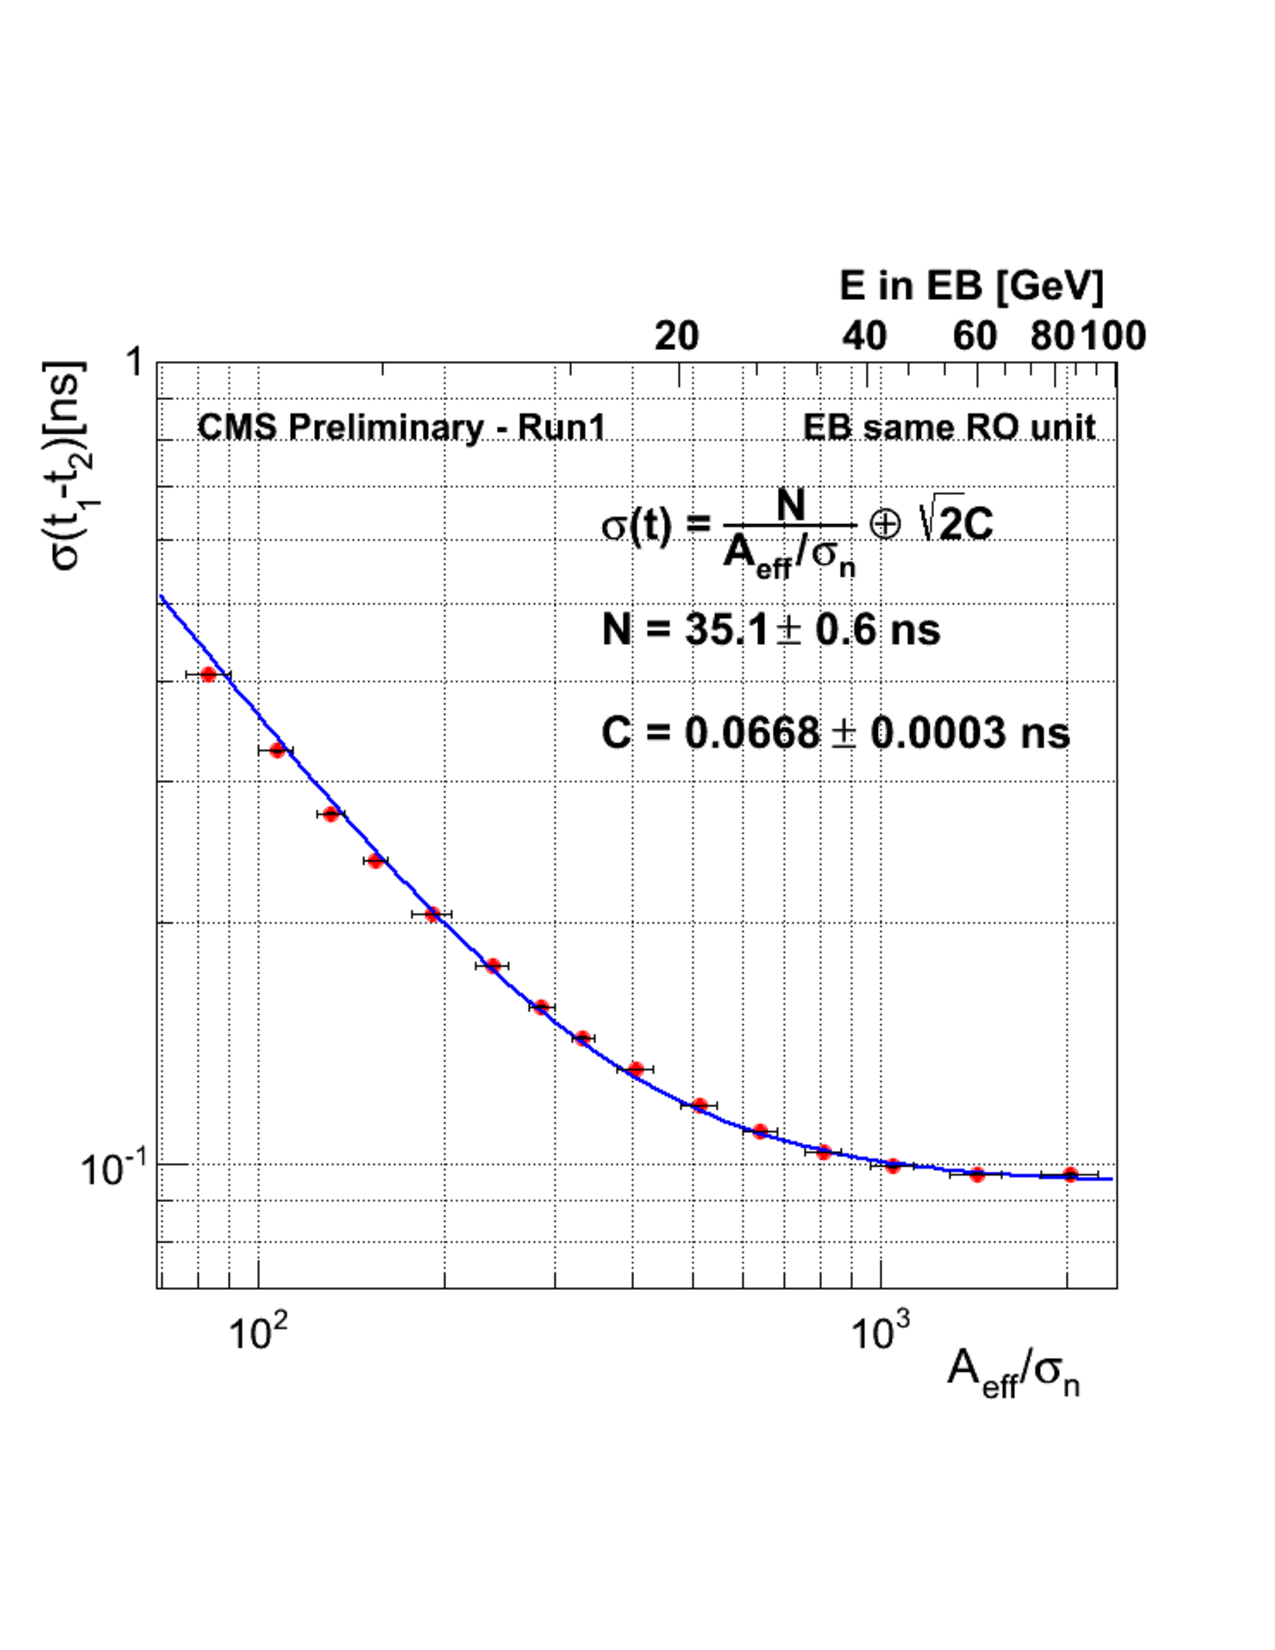
\includegraphics[height=0.8\textwidth, width=0.5\textwidth]{THESISPLOTS/TimeResSameElecCrystals.pdf}\quad
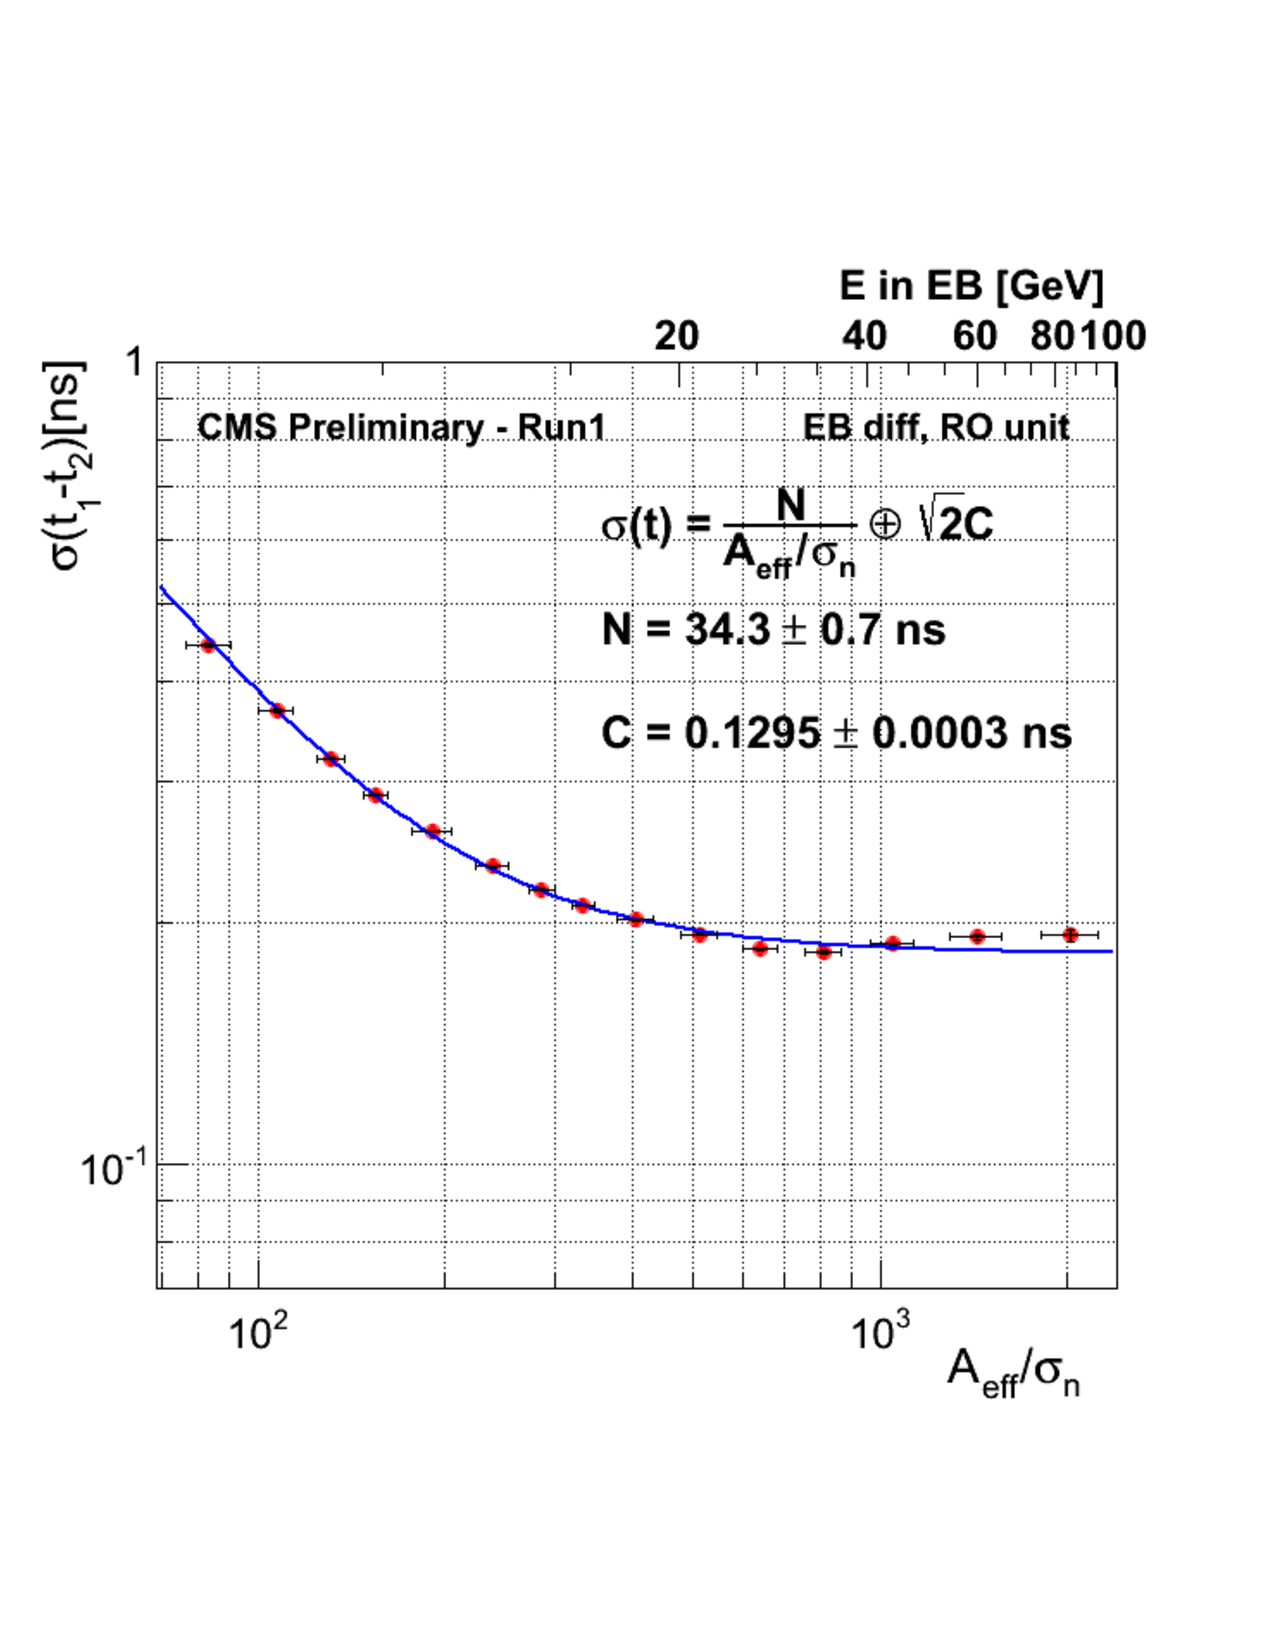
\includegraphics[height=0.8\textwidth, width=0.5\textwidth]{THESISPLOTS/TimeResDiffElecCrystals.pdf}}
\vspace{-2.5cm}
\captionof{figure}{ Timing resolution from:
\textit{left}: Two most energetic crystals in the same readout unit,
\textit{right}: Two most energetic crystals belonging to different readout units,
as a function of effective amplitude($A_{eff} = A_{1}A_{2}/\sqrt{A^{2}_{1} + A^{2}_{2}}$) normalized to noise in EB.
Both crystals are from reconstructed electrons in  $\PZ \rightarrow \Pelectron \Ppositron$ events.} 
\label{fig:ZeeTimeResolution}
%\end{figure}
\end{center}

%Table \ref{tab:TIMERes} shows ECAL timing resolution for 2011 and 2012 LHC Run 1. 
\begin{center}
%\begin{table}
\centering
 %\setlength{\abovecaptionskip}{0pt}
  %\setlength{\belowcaptionskip}{10pt}
 %\topcaption{GMSB,GGM Phenomenology and Relevant final states}
  \begin{tabular}{cc||lc} % p{0.1cm}|p{0.1cm}|}
  %\hline
 & \multicolumn{1}{r}{\bfseries{ECAL Timing Resolution}}\\
  \toprule
 & \multicolumn{2}{c}{\bfseries{2011}} \\
   \hline \hline
   & \vtop{\hbox{\strut{\bfseries{Absolute Time}}} \hbox{\strut{$\sigma_{eff}(t_{seed})$[ps]}} }  
   & \vtop{\hbox{\strut{\bfseries{Single Precision}}}\hbox{\strut{$\sigma_{eff}(t_{e1} - t_{e2})/\sqrt{2}$[ps]}} } \\ \hline
   \textbf{EB} & 376  & 190 \\
      \textbf{EE} & 356  & 282 \\
      \hline 
& \multicolumn{2}{c}{\bfseries{2012}}  \\
   \hline \hline
   &  \vtop{\hbox{\strut{\bfseries{Absolute Time}}}\hbox{\strut{$\sigma_{eff}(t_{seed})$[ps]}} }       
   &  \vtop{\hbox{\strut{\bfseries{Single Precision} }} \hbox{\strut{$\sigma_{eff}(t_{e1} - t_{e2})/\sqrt{2}$[ps]}} }  \\ \hline
   \textbf{EB} & 340  & 164 \\
      \textbf{EE} & 342  & 272 \\
      \hline
      \bottomrule
  \end{tabular}
   \captionof{table}{ECAL timing resolution absolute time and single precision for 2011 and 2012 of LHC Run 1}
 %\caption{ECAL timing resolution performances for 2011 and 2012 of LHC Run 1}
 \label{tab:TIMERes} % for use in \ref{table1} if you want to refer to the table number
\end{center}
%\end{table}
%\begin{center}
%\begin{tabular}{cc|c|c|c|c|l}
%\centering
%\cline{3-6}
%& & \multicolumn{4}{ c| }{Primes} \\ \cline{3-6}
%& & 2 & 3 & 5 & 7 \\ \cline{1-6}
%\multicolumn{1}{ |c| }{\multirow{2}{*}{Powers} } &
%\multicolumn{1}{ |c| }{504} & 3 & 2 & 0 & 1 &     \\ \cline{2-6}
%\multicolumn{1}{ |c  }{}                        &
%\multicolumn{1}{ |c| }{540} & 2 & 3 & 1 & 0 &     \\ \cline{1-6}
%\multicolumn{1}{ |c  }{\multirow{2}{*}{Powers} } &
%\multicolumn{1}{ |c| }{gcd} & 2 & 2 & 0 & 0 & min \\ \cline{2-6}
%\multicolumn{1}{ |c  }{}                        &
%\multicolumn{1}{ |c| }{lcm} & 3 & 3 & 1 & 1 & max \\ \cline{1-6}
%\end{tabular}
% \captionof{table}{Table Comparing Timing Resolution performance of 2011 Vs 2012}
% \label{tab:TIMERes} % for use in \ref{table1} if you want to refer to the table number
%\end{center}
%%%%%%%%%%%%%%%%%%%%%%%%%%%%%%%%%%%%%%%%%%%%%%
\label{ECAL Timing Calibration_chapter}
